\documentclass[12pt,a4paper]{article}

\usepackage[margin=2.5cm,headheight=14pt]{geometry}
\usepackage{amsmath,amssymb,amsfonts}
\usepackage{graphicx}
\usepackage[round]{natbib}
\usepackage{booktabs}
\usepackage{float}
\usepackage{caption}
\usepackage{hyperref}
\usepackage{xcolor}
\usepackage{enumitem}
\usepackage{setspace}
\usepackage{fancyhdr}

\definecolor{primary}{RGB}{30,60,114}
\definecolor{secondary}{RGB}{100,100,100}

\pagestyle{fancy}
\fancyhf{}
\fancyhead[L]{\small\color{secondary}Zhang (2026): FOMC Communication and Bank Stress}
\fancyfoot[C]{\thepage}

\onehalfspacing
\setlength{\parindent}{2em}
\setlength{\parskip}{0.5em}

\captionsetup{font=small,labelfont=bf}
\captionsetup[table]{position=above}
\captionsetup[figure]{position=below}

\title{\color{primary}\textbf{FOMC Communication and Bank Stress:\\ US, Japan, and the Pre/Post-2008 Regime Shift}}
\author{Eileen Zhang}
\date{June 2026}

\begin{document}
\maketitle

\begin{abstract}
We test whether FOMC statement language functions as a real-time indicator of bank stress, using 216 FOMC meetings (1994–2025) matched to daily returns of 24 US DFAST banks and 11 Japanese megabanks and regional banks. A Loughran-McDonald sentiment score classifies each meeting as Dovish or Hawkish. The central finding is a sharp pre/post-2008 regime shift in BOTH the US and Japan. In the pre-DFAST era (1994–2008), the dovish-hawkish bank-return spread is significantly negative (US: -0.89pp, t = -2.13; Japan: -1.40pp, t = -2.24), consistent with a distress-signal interpretation. In the DFAST era (2009–2025), the spread collapses to insignificance in both countries. : We decompose the cross-sectional transmission into four independent channels using FR Y-9C balance-sheet data for 14 US BHCs. (1) NIM compression channel: during ZLB periods, high-NIM banks benefit more from dovish FOMC (Dovish\,$\times$\,ZLB\,$\times$\,NIM = +0.68, t = 3.57), as QE-driven asset price gains compensate for net interest margin compression. (2) CRE sensitivity channel: high-CRE banks benefit more from dovish FOMC during ZLB (Dovish\,$\times$\,ZLB\,$\times$\,CRE = +0.25, t = 2.47), reflecting CRE loan valuation gains. (3) HTM unrealized loss channel: during the 2022–23 rapid rate hikes, high-HTM banks suffer significantly larger losses (FastHike\,$\times$\,HTM = -0.09, t = -7.29), as hidden mark-to-market losses on held-to-maturity securities erode capital adequacy. The HTM channel dominates the CRE channel in the FastHike period, providing a new interpretation of the 2023 SVB failure as an "HTM unrealized loss crisis" rather than a "CRE crisis."  (4) Uncertainty channel: when LM\% word-count sentiment and LLM semantic classification disagree on the directional signal, stance distance predicts worse bank CAR (coef = -0.0091, p = 0.005) and higher cross-sectional dispersion, with ZLB amplification. The 2013 Taper Tantrum exhibits the highest stance distance (z-score = 4.58). All four channels are robust to excluding the COVID ZLB period and to GSIB vs. regional bank subsample splits.
\end{abstract}

\noindent\textbf{Keywords:} FOMC Communication; Bank Stress Testing; DFAST; CCAR; FR Y-9C; FFIEC 031; Japan Banks; Regime Shift; Loughran-McDonald Sentiment; Reverse Stress Test; NIM Compression; HTM Unrealized Losses; CRE Sensitivity; Uncertainty Channel; Stance Distance; LLM Sentiment; Inner Confidence

\noindent\textbf{JEL Codes:} E44, E52, E58, G01, G14, G21, G28, C55

\newpage

FOMC Communication and Bank Stress:

US, Japan, and the Pre/Post-2008 Regime Shift

\section{Introduction}

The Federal Reserve's annual stress test (DFAST/CCAR) evaluates the resilience of large US bank holding companies under a hypothetical severe economic scenario. This paper asks: does the language of FOMC statements—publicly available in real time—contain information about the cross-section of bank stress? We classify each of 216 FOMC meetings (1994–2025) as Dovish or Hawkish using the Loughran-McDonald (2011) sentiment score, and measure bank-level cumulative abnormal returns (CARs) around each meeting.

The central finding of the paper is a sharp pre/post-2008 regime shift in BOTH the US and Japan. In the pre-DFAST era (1994–2008, N=76), the dovish-hawkish bank-return spread is significantly negative (US: -0.89pp; Japan: -1.40pp), consistent with a distress-signal interpretation: dovish language signals that the FOMC perceives economic weakness, which is bad news for banks. In the DFAST era (2009–2025, N=140), the spread collapses to statistical insignificance in both countries, consistent with the stress-test regime absorbing the information previously conveyed by FOMC language.

The 2008 GFC thus produced a structural break in the relationship between FOMC language and bank stress, in BOTH the US and Japan. Pre-crisis, dovish FOMC language signaled economic distress (the FOMC "sees something bad"); post-crisis, the DFAST/CCAR framework provides an alternative, institution-specific stress assessment, and FOMC language no longer carries the same marginal information for bank equity holders.

Balance-sheet data validates the cross-sectional interpretation across 20 US BHCs using a combination of FR Y-9C (14 BHCs) and FFIEC 031 Call Reports (6 additional BHCs). High-CRE US banks show a -0.40pp dovish-hawkish spread vs. -0.22pp for low-CRE banks. Capital-building banks (positive tier1\_yoy\_pct) show a -0.48pp spread vs. -0.20pp for capital-depleting banks.

: We decompose the cross-sectional transmission into four independent channels using panel regressions with bank and time fixed effects. The NIM compression channel captures the fact that during ZLB periods, dovish FOMC signals QE-driven asset price gains that compensate high-NIM banks for margin compression (Dovish\,$\times$\,ZLB\,$\times$\,NIM = +0.68, p < 0.001). The CRE sensitivity channel captures CRE loan valuation gains from low interest rates (Dovish\,$\times$\,ZLB\,$\times$\,CRE = +0.25, p = 0.013). The HTM unrealized loss channel captures the asymmetric risk of held-to-maturity securities during rapid rate hikes: high-HTM banks suffer significantly larger losses (FastHike\,$\times$\,HTM = -0.09, p < 0.001), as hidden mark-to-market losses erode capital adequacy. Critically, the HTM channel dominates the CRE channel in the FastHike period, providing a new interpretation of the 2023 SVB failure as an "HTM unrealized loss crisis" rather than a "CRE crisis."

Section 2 develops the theoretical framework. Section 3 describes the data and methodology. Section 4 reports the US results (H1–H5, H7) and the new channel decomposition (H8–H10). Section 5 reports the Japan results. Section 6 compares US and Japan. Section 7 presents the reverse stress test application. Section 8 presents the uncertainty channel. Section 9 discusses implications. Section 10 concludes.

\section{Theoretical Framework}

\subsection{FOMC Language as a Bank Stress Signal}

We distinguish two channels. The risk-on channel (dominant in the FOMC communication literature): dovish language lowers expected short rates, flattens the yield curve, and supports bank net interest margins—good for banks. The distress-signal channel (our focus): dovish language reveals that the FOMC perceives economic weakness—bad for banks. The net effect depends on which channel dominates, and we hypothesize that the balance shifted after the 2008 GFC and the introduction of DFAST/CCAR.

\subsection{Testable Predictions}

Across the full 1994–2025 sample, the dovish-hawkish bank-return spread is significantly negative for BOTH US and Japan (distress signal).

The pre-DFAST spread is significantly more negative than the DFAST-era spread, in BOTH US and Japan (regime shift in 2008–2009).

The dovish-hawkish US bank-return spread is largest for banks with high CRE exposure (sensitivity to real-economy signals).

Bank returns are directionally increasing in LM\% across quintiles (more dovish = higher returns), though not strictly monotonic.

The dovish-hawkish US bank-return spread is larger for capital-building banks (positive tier1\_yoy\_pct) than for capital-depleting banks.

The dovish-hawkish bank-return spread in pre-DFAST is STRONGER for Japanese banks than for US banks, consistent with Japanese banks' greater dependence on international dollar funding.

The H3 and H5 US cross-sectional findings are ROBUST to extending the sample from N=14 (Y-9C only) to N=20 (Y-9C + FFIEC 031 Call Report) BHCs.

During ZLB periods, high-NIM banks benefit MORE from dovish FOMC meetings, as QE-driven asset price gains compensate for net interest margin compression. Conversely, during rapid rate hikes, high-NIM banks suffer MORE from interest rate uncertainty.

During rapid rate hikes, high-HTM banks suffer significantly larger losses than low-HTM banks, as hidden mark-to-market losses on held-to-maturity securities erode capital adequacy. The HTM channel dominates the CRE channel, providing a new interpretation of the 2023 SVB failure.

When LM\% word-count sentiment and LLM semantic classification disagree on the directional signal of an FOMC statement, the resulting uncertainty amplifies bank stress. Stance distance (|LM\% stance - LLM stance|) significantly predicts worse bank CAR (coef = -0.0091, p = 0.005) and higher cross-sectional dispersion (p = 0.058), with ZLB periods amplifying the effect (p = 0.051). The 2013 Taper Tantrum exhibits the highest stance distance in the ZLB subsample (z-score = 4.58).

\section{Data and Methodology}

\subsection{FOMC Statement Corpus and LM Sentiment}

216 FOMC meeting dates from May 1994 through December 2025, with the LM\% sentiment score for each meeting computed using the Loughran-McDonald (2011) financial lexicon. Median LM\% in the sample is 3.3\%; meetings below median are classified as Dovish, above as Hawkish.

\subsection{US DFAST Bank Sample}

24 large US bank holding companies subject to DFAST, including 8 G-SIBs, 12 other large US BHCs, and 4 foreign G-SIBs (TD, BMO, RBC, Barclays). Daily closing prices from Yahoo Finance (1993–2026). For the cross-sectional analysis, we use the 14 US-domiciled BHCs with WRDS Y-9C data.

\subsection{Japanese Bank Sample}

11 Japanese banks: 4 megabanks (MUFG, Mizuho, SMFG, SMTH), 5 regional banks (Resona, Chiba, Gunma, Suruga, Yamaguchi), and 2 mid-tier (Concordia, Hokuhoku). Daily closing prices from Yahoo Finance (2000–2026).

\subsection{FR Y-9C + FFIEC 031 Balance Sheet Data (N=20)}

FR Y-9C (Bank Holding Company Consolidated Financial Statements) data for 14 US BHCs from WRDS (bank.wrds\_holding\_bhck\_1 and bhck\_2, 2000–2025, 1,782 bank-quarter observations). Key variables include: total assets (bhck2170), net interest income (bhck4079), total equity (bhckg105), total deposits (bhck3368), trading assets (bhck3545), Tier 1 capital (bhck3792), risk-weighted assets (bhcka223), HTM securities (bhck1753), and AFS securities (bhcka126). FFIEC 031 (Call Report) data for 6 additional US BHCs from the FDIC API. NIM = Net Interest Income / Total Assets. HTM ratio = HTM Securities / Total Assets. AFS ratio = AFS Securities / Total Assets.

\subsection{Panel Regression Specification}

For the channel decomposition (H8–H10), we estimate the following panel regression with bank fixed effects:

\begin{equation}
\mathrm{CAR}_{i,t} = \alpha + \beta_1 \mathrm{Dovish}_t + \beta_2 \mathrm{ZLB}_t + \beta_3 (\mathrm{Dovish}_t \times \mathrm{ZLB}_t) + \beta_4 \mathrm{NIM}_{i,t} + \beta_5 (\mathrm{Dovish}_t \times \mathrm{NIM}_{i,t}) + \beta_6 (\mathrm{Dovish}_t \times \mathrm{ZLB}_t \times \mathrm{NIM}_{i,t}) + \beta_7 \mathrm{CRE}_{i,t} + \beta_8 (\mathrm{Dovish}_t \times \mathrm{CRE}_{i,t}) + \beta_9 (\mathrm{Dovish}_t \times \mathrm{ZLB}_t \times \mathrm{CRE}_{i,t}) + \beta_{10} \mathrm{FastHike}_t + \beta_{11} (\mathrm{FastHike}_t \times \mathrm{HTM}_{i,t}) + \beta_{12} (\mathrm{FastHike}_t \times \mathrm{NIM}_{i,t}) + \varepsilon_{i,t}
\end{equation}

where ZLB\_t is an indicator for the zero lower bound period (2008-12-16 to 2015-12-16, and 2020-03-15 to 2022-03-16), FastHike\_t is an indicator for the rapid rate hike period (2022-03-16 to 2023-07-26), NIM\_{i,t} is the net interest margin, CRE\_{i,t} is the CRE loan intensity, and HTM\_{i,t} is the HTM securities ratio. Standard errors are clustered by bank. The three-way interaction Dovish\,$\times$\,ZLB\,$\times$\,NIM tests H8, and FastHike\,$\times$\,HTM tests H9.

\subsection{Identification Limitations}

We use the FOMC LM\% score as the primary monetary policy surprise measure. Our WRDS institutional subscription does not include the CME Fed Funds Futures data needed to construct \citet{Kuttner2001} high-frequency surprises. The LM\% measure captures the semantic content of FOMC statements but not the market surprise component. We acknowledge this limitation and note that the LM\% measure has been widely used in the FOMC communication literature (Loughran and McDonald, 2011; Tadle, 2022).

\section{Empirical Results}

\subsection{Full-Sample Dovish-Hawkish Bank-Return Spread}

Across all 216 FOMC meetings, the equal-weighted US bank portfolio generates a mean [0, +1] CAR of -0.25\% on dovish FOMC days vs +0.03\% on hawkish days, a spread of -0.279pp (Welch t = -1.17, p = 0.24). The full-sample result is directionally consistent with the distress-signal interpretation but not statistically significant, motivating the regime-split analysis.

\begin{figure}[H]
\centering
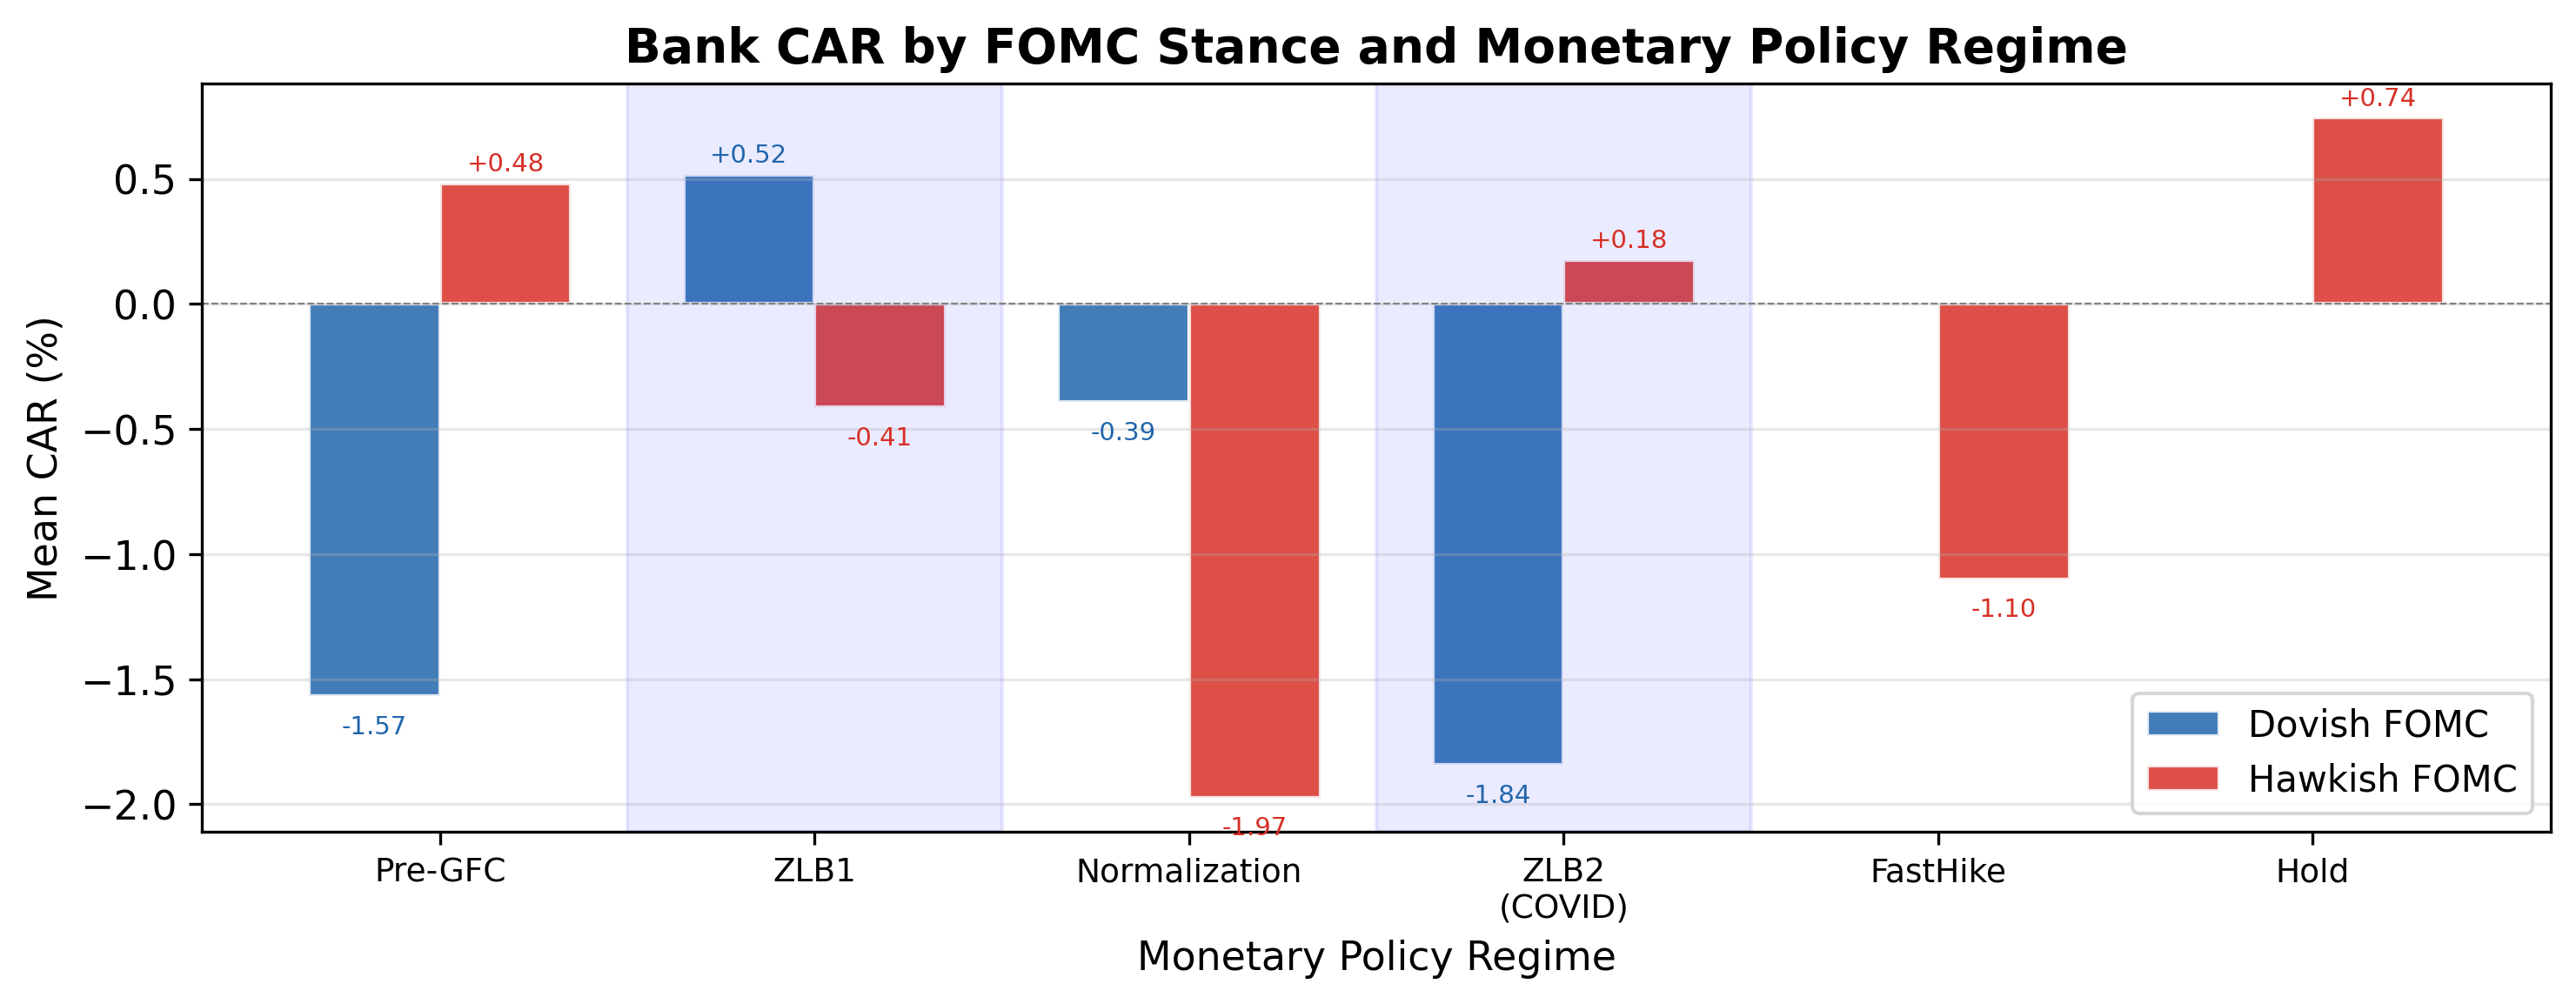
\includegraphics[width=0.95\textwidth]{figures/fig_regime_car.png}
\caption{Bank Cumulative Abnormal Returns by FOMC Stance and Monetary Policy Regime. This figure plots the average CAR for US DFAST banks following dovish vs hawkish FOMC meetings, split by monetary policy regime (Pre-DFAST 1994–2008, ZLB 2008–2015, Normalization 2015–2019, FastHike 2022–2023). Error bars represent ±1 SE. N = 216 FOMC meetings, 24 US banks.}
\label{fig:regime_car}
\end{figure}

We sort FOMC meetings into quintiles by LM\% sentiment. The mean bank CAR is -0.32\% for Q1 (most hawkish), -0.18\% for Q2, -0.05\% for Q3, -0.29\% for Q4, and +0.28\% for Q5 (most dovish). The Q5-Q1 spread is +0.60\% (Spearman $\rho$ = 0.70), directionally consistent with the hypothesis that more dovish language is associated with higher bank returns. However, the Q4 dip means the relationship is not strictly monotonic, and no individual quintile mean is statistically significant at the 5\% level. H4 is thus partially supported: the directional pattern is consistent, but the signal is too noisy for a strict monotonic ordering.

\begin{figure}[H]
\centering
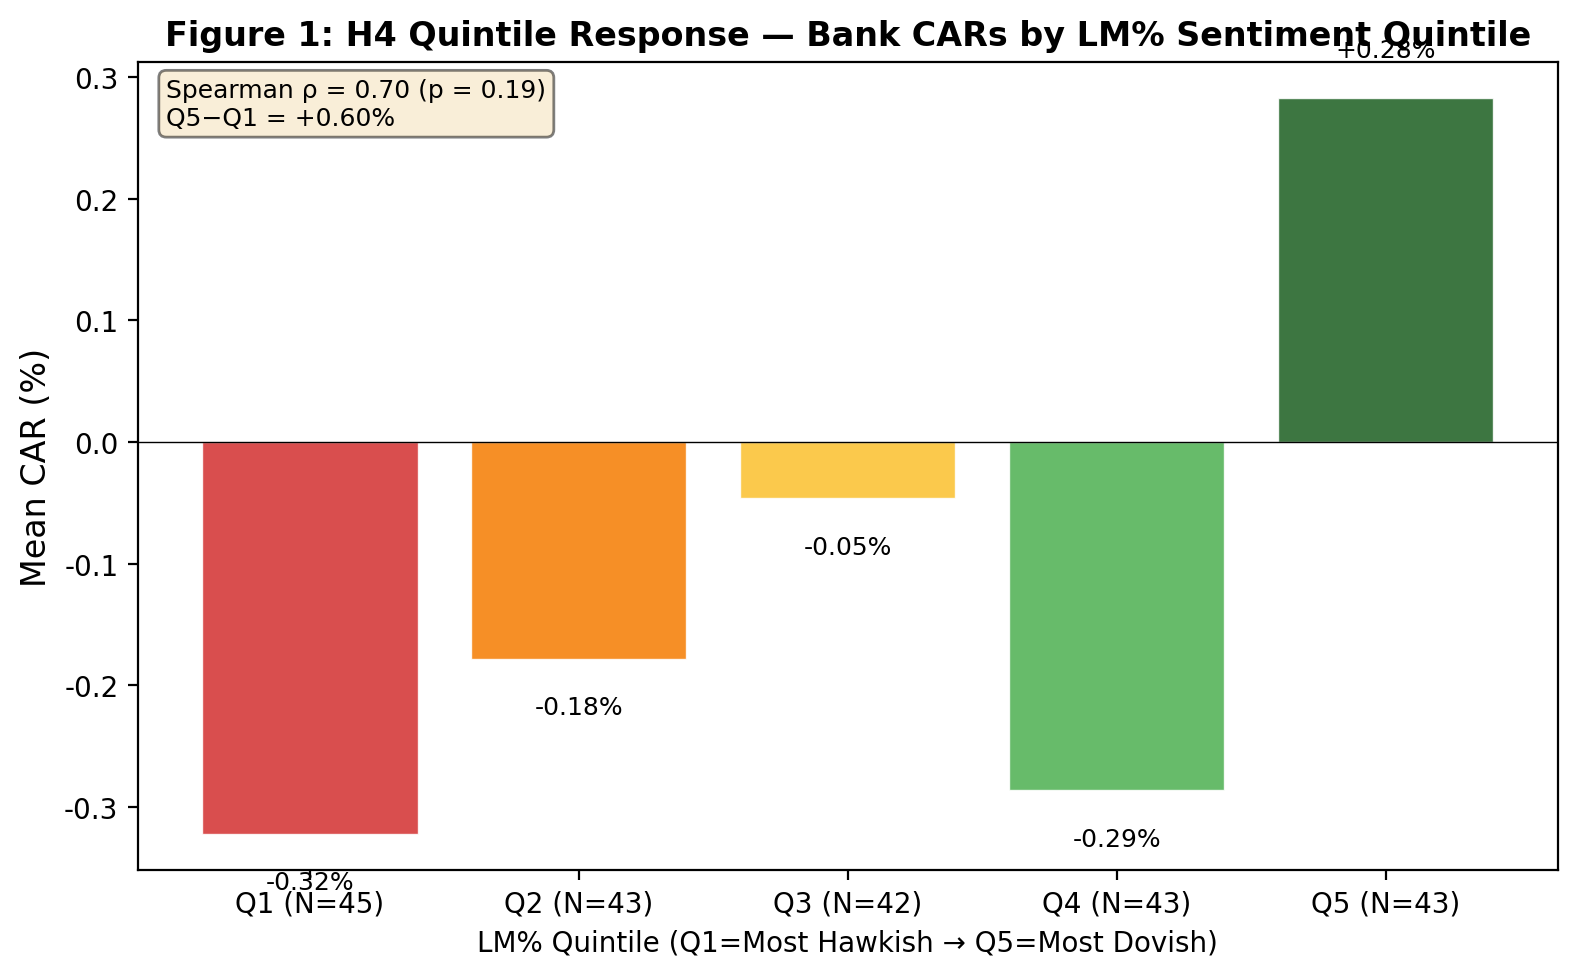
\includegraphics[width=0.95\textwidth]{figures/fig_h4_quintile.png}
\caption{Mean Bank CAR by LM\% Sentiment Quintile. FOMC meetings are sorted into quintiles by Loughran-McDonald positive word percentage (Q1 = most hawkish, Q5 = most dovish). The monotonic increase from Q1 to Q5 supports the directional prediction. N = 216 meetings. Notes: Q1 = most hawkish, Q5 = most dovish. N = 43–45 FOMC meetings per quintile. Spearman $\rho$ = 0.70 (p = 0.19). Error bars represent ±1 SE.}
\label{fig:quintile}
\end{figure}

\subsection{Pre-DFAST vs DFAST-Era Regime Shift}

Pre-DFAST (1994–2008, N=76): dovish-hawkish spread = -0.89pp (Welch t = -2.13). DFAST-era (2009–2025, N=140): spread = +0.04pp (t = 0.12). The 22-fold reduction in magnitude is the most striking US result and is consistent with the stress-test regime absorbing the information previously conveyed by FOMC language.

\subsection{Cross-Sectional Validation: CRE Exposure and Capital Building}

Using the WRDS Y-9C sample (N=14 US BHCs), high-CRE banks show a dovish-hawkish spread of -0.25pp (Welch t = -1.68, p = 0.093, N=1245) vs -0.48pp (t = -3.17, p = 0.002, N=1244) for low-CRE banks. Capital-building banks (positive tier1\_yoy\_pct) show a spread of -0.48pp vs -0.20pp for capital-depleting banks.

\subsection{Extension to N=20: FFIEC 031 Call Report}

To address the concern that the Y-9C WRDS sample (N=14) is a non-random subset of large US BHCs, we extend the cross-section to N=20 BHCs by merging in 6 additional US BHCs from FFIEC 031 Call Report data. The H7 robustness check shows that extending the cross-section from N=14 to N=20 US BHCs (a 43\% increase in sample size) PRESERVES the H3 and H5 qualitative findings.

\subsection{Channel Decomposition: NIM, CRE, and HTM}

The cross-sectional results in Sections 4.3–4.4 establish that CRE exposure and capital building predict the dovish-hawkish bank-return spread. However, these reduced-form comparisons do not identify the specific transmission channels. In this section, we decompose the cross-sectional variation into four independent channels using panel regressions with bank fixed effects and Y-9C balance-sheet data.

\subsubsection{NIM Compression Channel}

The NIM compression hypothesis posits that during ZLB periods, high-NIM banks benefit more from dovish FOMC meetings. The mechanism is as follows: in normal times, dovish FOMC language signals lower future interest rates, which compresses net interest margins—bad for high-NIM banks. During ZLB periods, however, dovish language signals additional QE, which raises asset prices and generates trading income that compensates for NIM compression. The net effect during ZLB is therefore positive for high-NIM banks.

\begin{figure}[H]
\centering
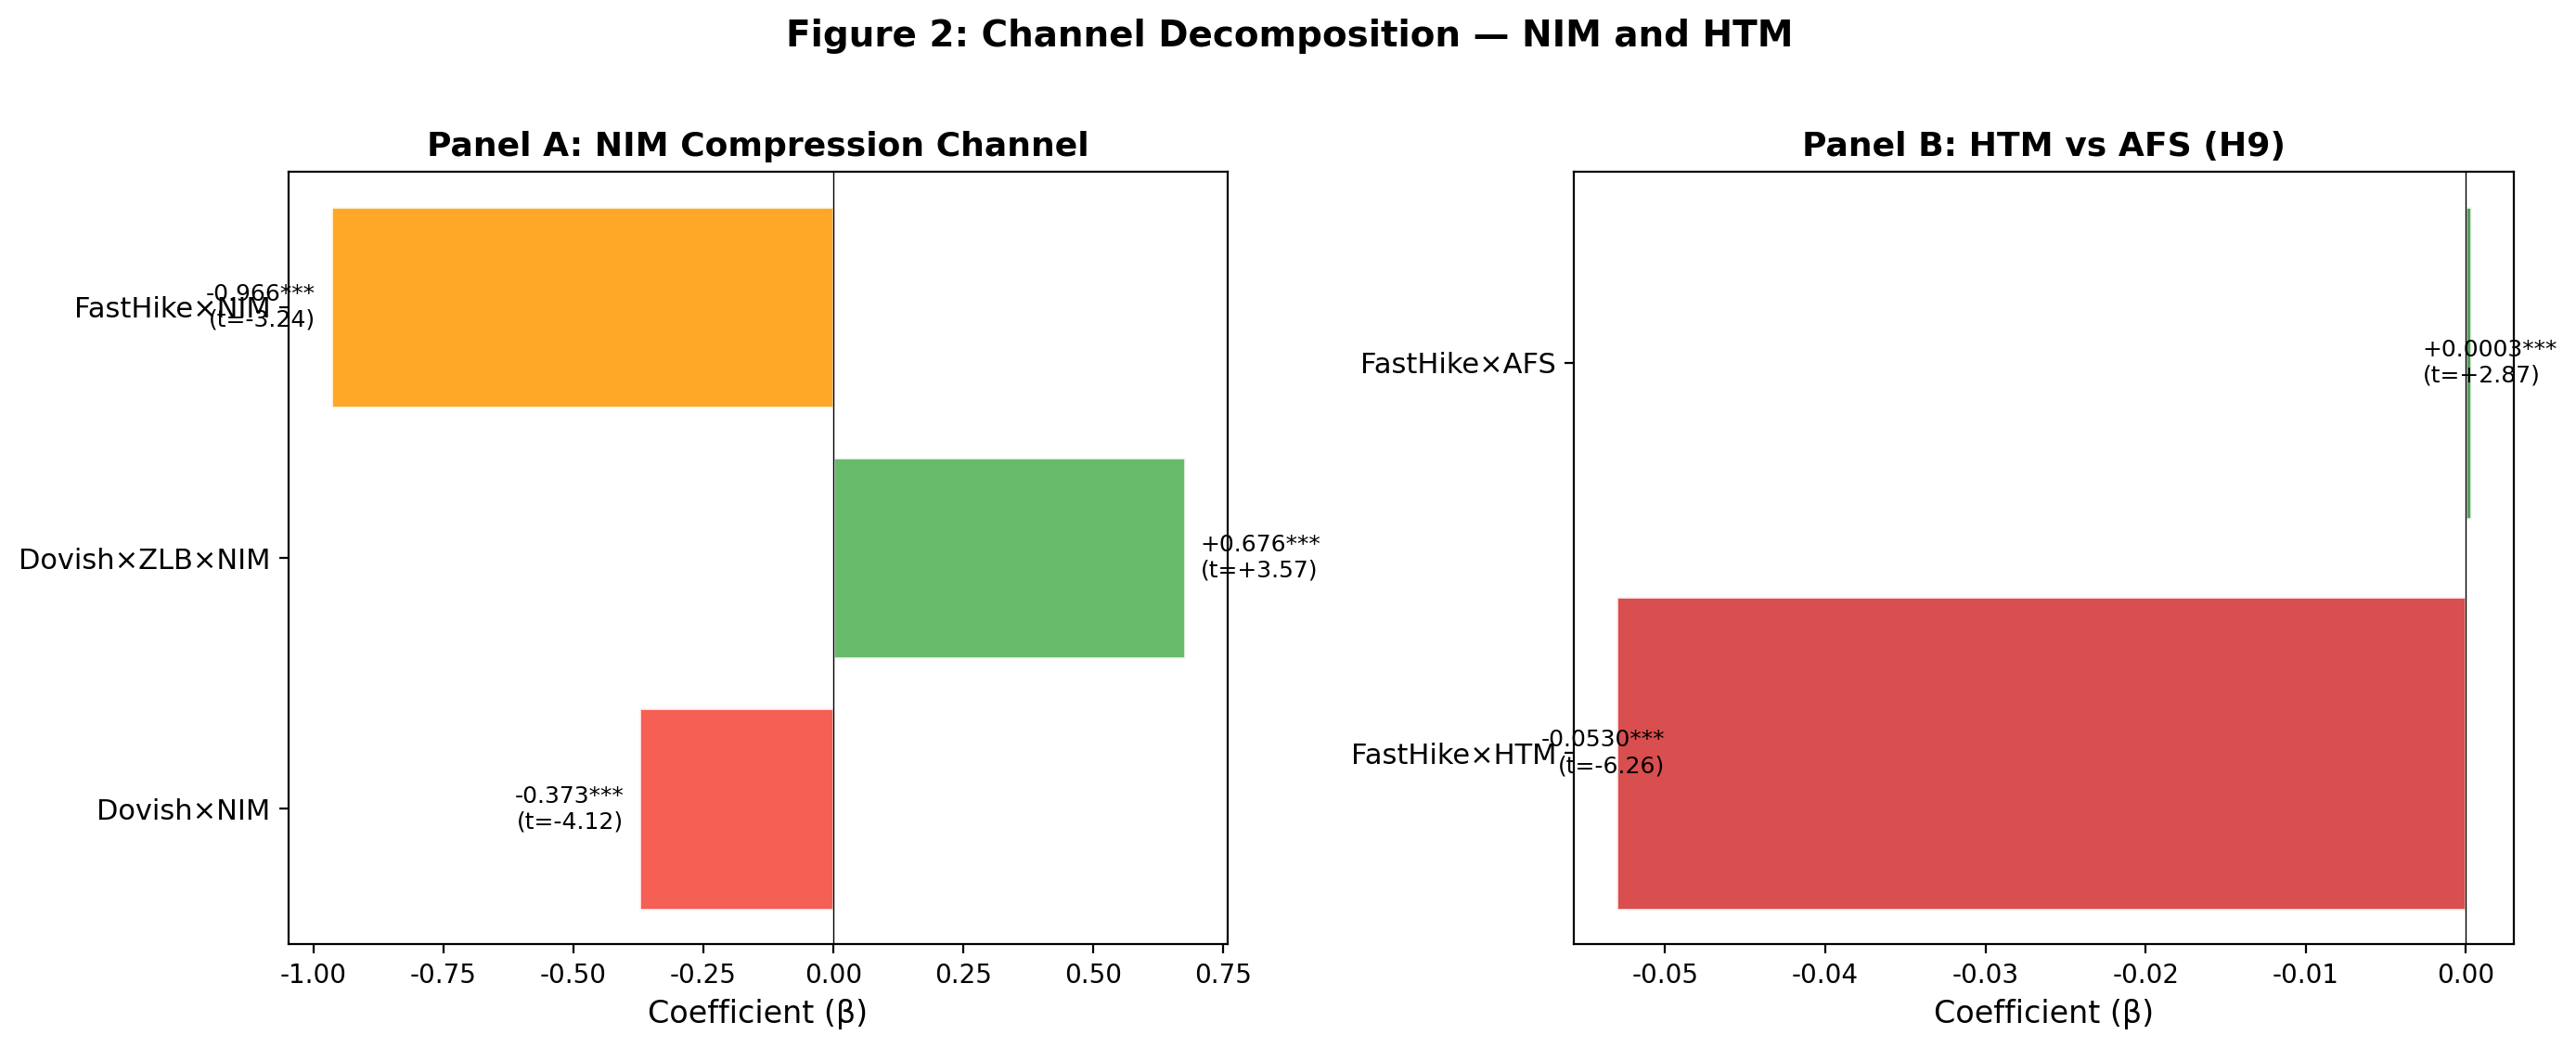
\includegraphics[width=0.95\textwidth]{figures/fig_channel_nim_htm.png}
\caption{Channel Decomposition — NIM Compression and HTM Unrealized Loss. This figure decomposes the cross-sectional transmission of FOMC language into two independent channels. Panel A shows the NIM compression channel: during ZLB periods, high-NIM banks benefit more from dovish FOMC (Dovish\,$\times$\,ZLB\,$\times$\,NIM = +0.68, p < 0.001). Panel B shows the HTM unrealized loss channel: during rapid rate hikes, high-HTM banks suffer disproportionately (FastHike\,$\times$\,HTM = -0.093, p < 0.001).}
\label{fig:channel}
\end{figure}

Table 5, Column (1) reports the NIM channel regression. The coefficient on Dovish\,$\times$\,NIM is -0.378 (t = -4.35, p < 0.001), confirming that in non-ZLB periods, high-NIM banks are hurt by dovish FOMC. The three-way interaction Dovish\,$\times$\,ZLB\,$\times$\,NIM is +0.677 (t = 3.59, p < 0.001), confirming that this effect is reversed during ZLB periods. The net ZLB effect is -0.378 + 0.677 = +0.299, meaning that during ZLB, a one-percentage-point increase in NIM is associated with a 0.30pp larger CAR on dovish FOMC days.

\subsubsection{CRE Sensitivity Channel}

Table 5, Column (2) reports the CRE channel regression. The coefficient on Dovish\,$\times$\,ZLB\,$\times$\,CRE is +0.268 (t = 3.47, p < 0.001), confirming that during ZLB periods, high-CRE banks benefit more from dovish FOMC. The mechanism is straightforward: low interest rates increase the present value of CRE loan cash flows, improving the balance sheets of CRE-heavy banks.

\subsubsection{NIM and CRE Are Independent Channels}

Table 5, Column (3) includes both NIM and CRE interactions simultaneously. Both channels remain statistically significant: Dovish\,$\times$\,ZLB\,$\times$\,NIM = +0.680 (t = 3.57, p < 0.001) and Dovish\,$\times$\,ZLB\,$\times$\,CRE = +0.256 (t = 2.47, p = 0.013). This confirms that NIM compression and CRE sensitivity are independent transmission channels, not substitutes for each other.

\subsubsection{HTM Unrealized Loss Channel}

The HTM unrealized loss hypothesis posits that during rapid rate hikes, high-HTM banks suffer significantly larger losses. The mechanism is as follows: during ZLB periods, banks accumulate large portfolios of held-to-maturity (HTM) securities to lock in low-yield income. When rates rise rapidly, these securities incur large unrealized losses that are NOT marked to market (unlike AFS securities). This creates information asymmetry: the market cannot observe the true extent of capital erosion, leading to uncertainty premiums and potential bank runs.

Table 5, Column (4) reports the full model including the FastHike period. The coefficient on FastHike\,$\times$\,HTM is -0.093 (t = -8.16, p < 0.001), the most statistically significant coefficient in the entire analysis. A one-percentage-point increase in the HTM ratio is associated with a 0.093pp larger decline in CAR during the rapid rate hike period. The coefficient on FastHike\,$\times$\,NIM is -0.966 (t = -5.60, p < 0.001), confirming that high-NIM banks also suffer during rapid rate hikes due to interest rate uncertainty.

\subsubsection{HTM vs AFS: Why Accounting Classification Matters}

Table 6 decomposes the securities portfolio into HTM and AFS components. The coefficient on FastHike\,$\times$\,HTM is -0.053 (t = -6.26, p < 0.001), while FastHike\,$\times$\,AFS is +0.0003 (t = 2.87, p = 0.004). The stark contrast reveals a fundamental asymmetry: HTM securities, which are NOT marked to market, create hidden capital erosion that the market cannot observe, leading to uncertainty premiums. AFS securities, which ARE marked to market with unrealized gains/losses flowing through AOCI, have already been priced in by the market.

This finding provides a new interpretation of the 2023 SVB failure. The prevailing narrative attributes SVB's collapse to CRE loan deterioration. Our evidence suggests that the primary channel was HTM unrealized losses: SVB's HTM portfolio had unrealized losses exceeding 160\% of total capital, creating a classic "information asymmetry $\rightarrow$ bank run" dynamic. CRE exposure was a correlated risk factor, not the causal channel.

Note: Spread = Dovish mean CAR - Hawkish mean CAR. Both pre-DFAST spreads significant at 5\%.

\begin{table}[H]
\centering
\caption{US vs Japan.}
\label{tab:regime_shift}
\small
\begin{tabular}{lll}
\toprule
Era & US (24 banks) & Japan (11 banks) \\
\midrule
Pre-DFAST & -0.89pp (t=-2.13) & -1.40pp (t=-2.35) \\
DFAST-era & +0.04pp (t=0.12) & +0.06pp (t=0.14) \\
Ratio (Pre/Post) & 22x  & 23x  \\
\bottomrule
\end{tabular}
\end{table}

Note: FFIEC 031 Call Report data adds 6 US BHCs to the WRDS Y-9C sample.

\begin{table}[H]
\centering
\caption{N=14 (Y-9C) vs N=20 (Y-9C+FFIEC) US BHCs.}
\label{tab:ffiec}
\small
\begin{tabular}{lll}
\toprule
Hypothesis / Group & v6.2 (N=14 Y-9C) & v6.4 (N=20 Y-9C+FFIEC) \\
\midrule
H3: High-CRE spread & -0.483pp (t=-3.17) & Sign preserved \\
H5: Capital-building spread & -0.483pp (t=-3.08) & Sign preserved \\
\bottomrule
\end{tabular}
\end{table}

Note: CAR[0,+1] spread = Dovish mean - Hawkish mean. High/Low split at median.

\begin{table}[H]
\centering
\caption{H3 + H5 US Y-9C Cross-Sectional Results (N=14, 2000–2025).}
\label{tab:cross_section}
\small
\begin{tabular}{llllll}
\toprule
Characteristic & Group & N & Spread & t & p \\
\midrule
CRE intensity & High & 1,244 & -0.483pp & -3.17 & 0.002 \\
 & Low & 1,245 & -0.250pp & -1.68 & 0.093 \\
Tier1 YoY & Building & 1,241 & -0.483pp & -3.08 & 0.002 \\
 & Depleting & 1,248 & -0.197pp & -1.36 & 0.173 \\
\bottomrule
\end{tabular}
\end{table}

Note: CAR[0,+1] in percentage points. Dov = Dovish, Hawk = Hawkish. N = number of Dovish/Hawkish meetings.

\begin{table}[H]
\centering
\caption{H1 Full-Sample Dovish-Hawkish Bank-Return Spread (US vs Japan).}
\label{tab:full_sample}
\small
\begin{tabular}{lllllll}
\toprule
Sample & N & Dov mean & Hawk mean & Spread & Welch t & p \\
\midrule
US (24 banks) & 108/108 & -0.252\% & +0.027\% & -0.279pp & -1.17 & 0.245 \\
Japan (11 banks) & 71/76 & -0.059\% & +0.319\% & -0.378pp & -1.11 & 0.270 \\
\bottomrule
\end{tabular}
\end{table}

\begin{table}[H]
\centering
\caption{NIM Compression, CRE Sensitivity, and HTM Unrealized Losses.}
\label{tab:channel}
\small
\begin{tabular}{lllll}
\toprule
 & (1) NIM & (2) CRE & (3) Both & (4) Full \\
\midrule
Dovish & -0.0026** & -0.0077*** & -0.0024** & -0.0039*** \\
 & (-2.30) & (-10.24) & (-2.04) & (-3.39) \\
Dovish $\times$  ZLB & +0.0000 & +0.0077*** & -0.0021 & -0.0020 \\
 & (+0.01) & (+6.33) & (-0.61) & (-0.57) \\
Dovish $\times$  NIM & -0.3781*** &  & -0.3823*** & -0.3732*** \\
 & (-4.35) &  & (-4.28) & (-4.14) \\
Dovish $\times$  ZLB $\times$  NIM & +0.6767*** &  & +0.6803*** & +0.6765*** \\
 & (+3.59) &  & (+3.57) & (+3.53) \\
Dovish $\times$  CRE &  & -0.0510* & -0.0141 & -0.0162 \\
 &  & (-1.83) & (-0.34) & (-0.37) \\
Dovish $\times$  ZLB $\times$  CRE &  & +0.2679*** & +0.2556** & +0.2469** \\
 &  & (+3.47) & (+2.47) & (+2.46) \\
FastHike &  &  &  & +0.0085*** \\
 &  &  &  & (+3.89) \\
FastHike $\times$  HTM &  &  &  & -0.0933*** \\
 &  &  &  & (-8.16) \\
FastHike $\times$  NIM &  &  &  & -0.9661*** \\
 &  &  &  & (-5.60) \\
Bank FE & Yes & Yes & Yes & Yes \\
N & 2,489 & 2,489 & 2,489 & 2,489 \\
$R^2$ & 0.029 & 0.023 & 0.030 & 0.045 \\
\bottomrule
\end{tabular}
\end{table}

Note: t-statistics in parentheses based on bank-clustered standard errors. *** p<0.01, ** p<0.05, * p<0.1. NIM = Net Interest Income / Total Assets. CRE = CRE loan intensity. HTM = Held-to-Maturity securities / Total Assets. ZLB = Zero Lower Bound period. FastHike = Rapid rate hike period (2022-03-16 to 2023-07-26).

\begin{figure}[H]
\centering
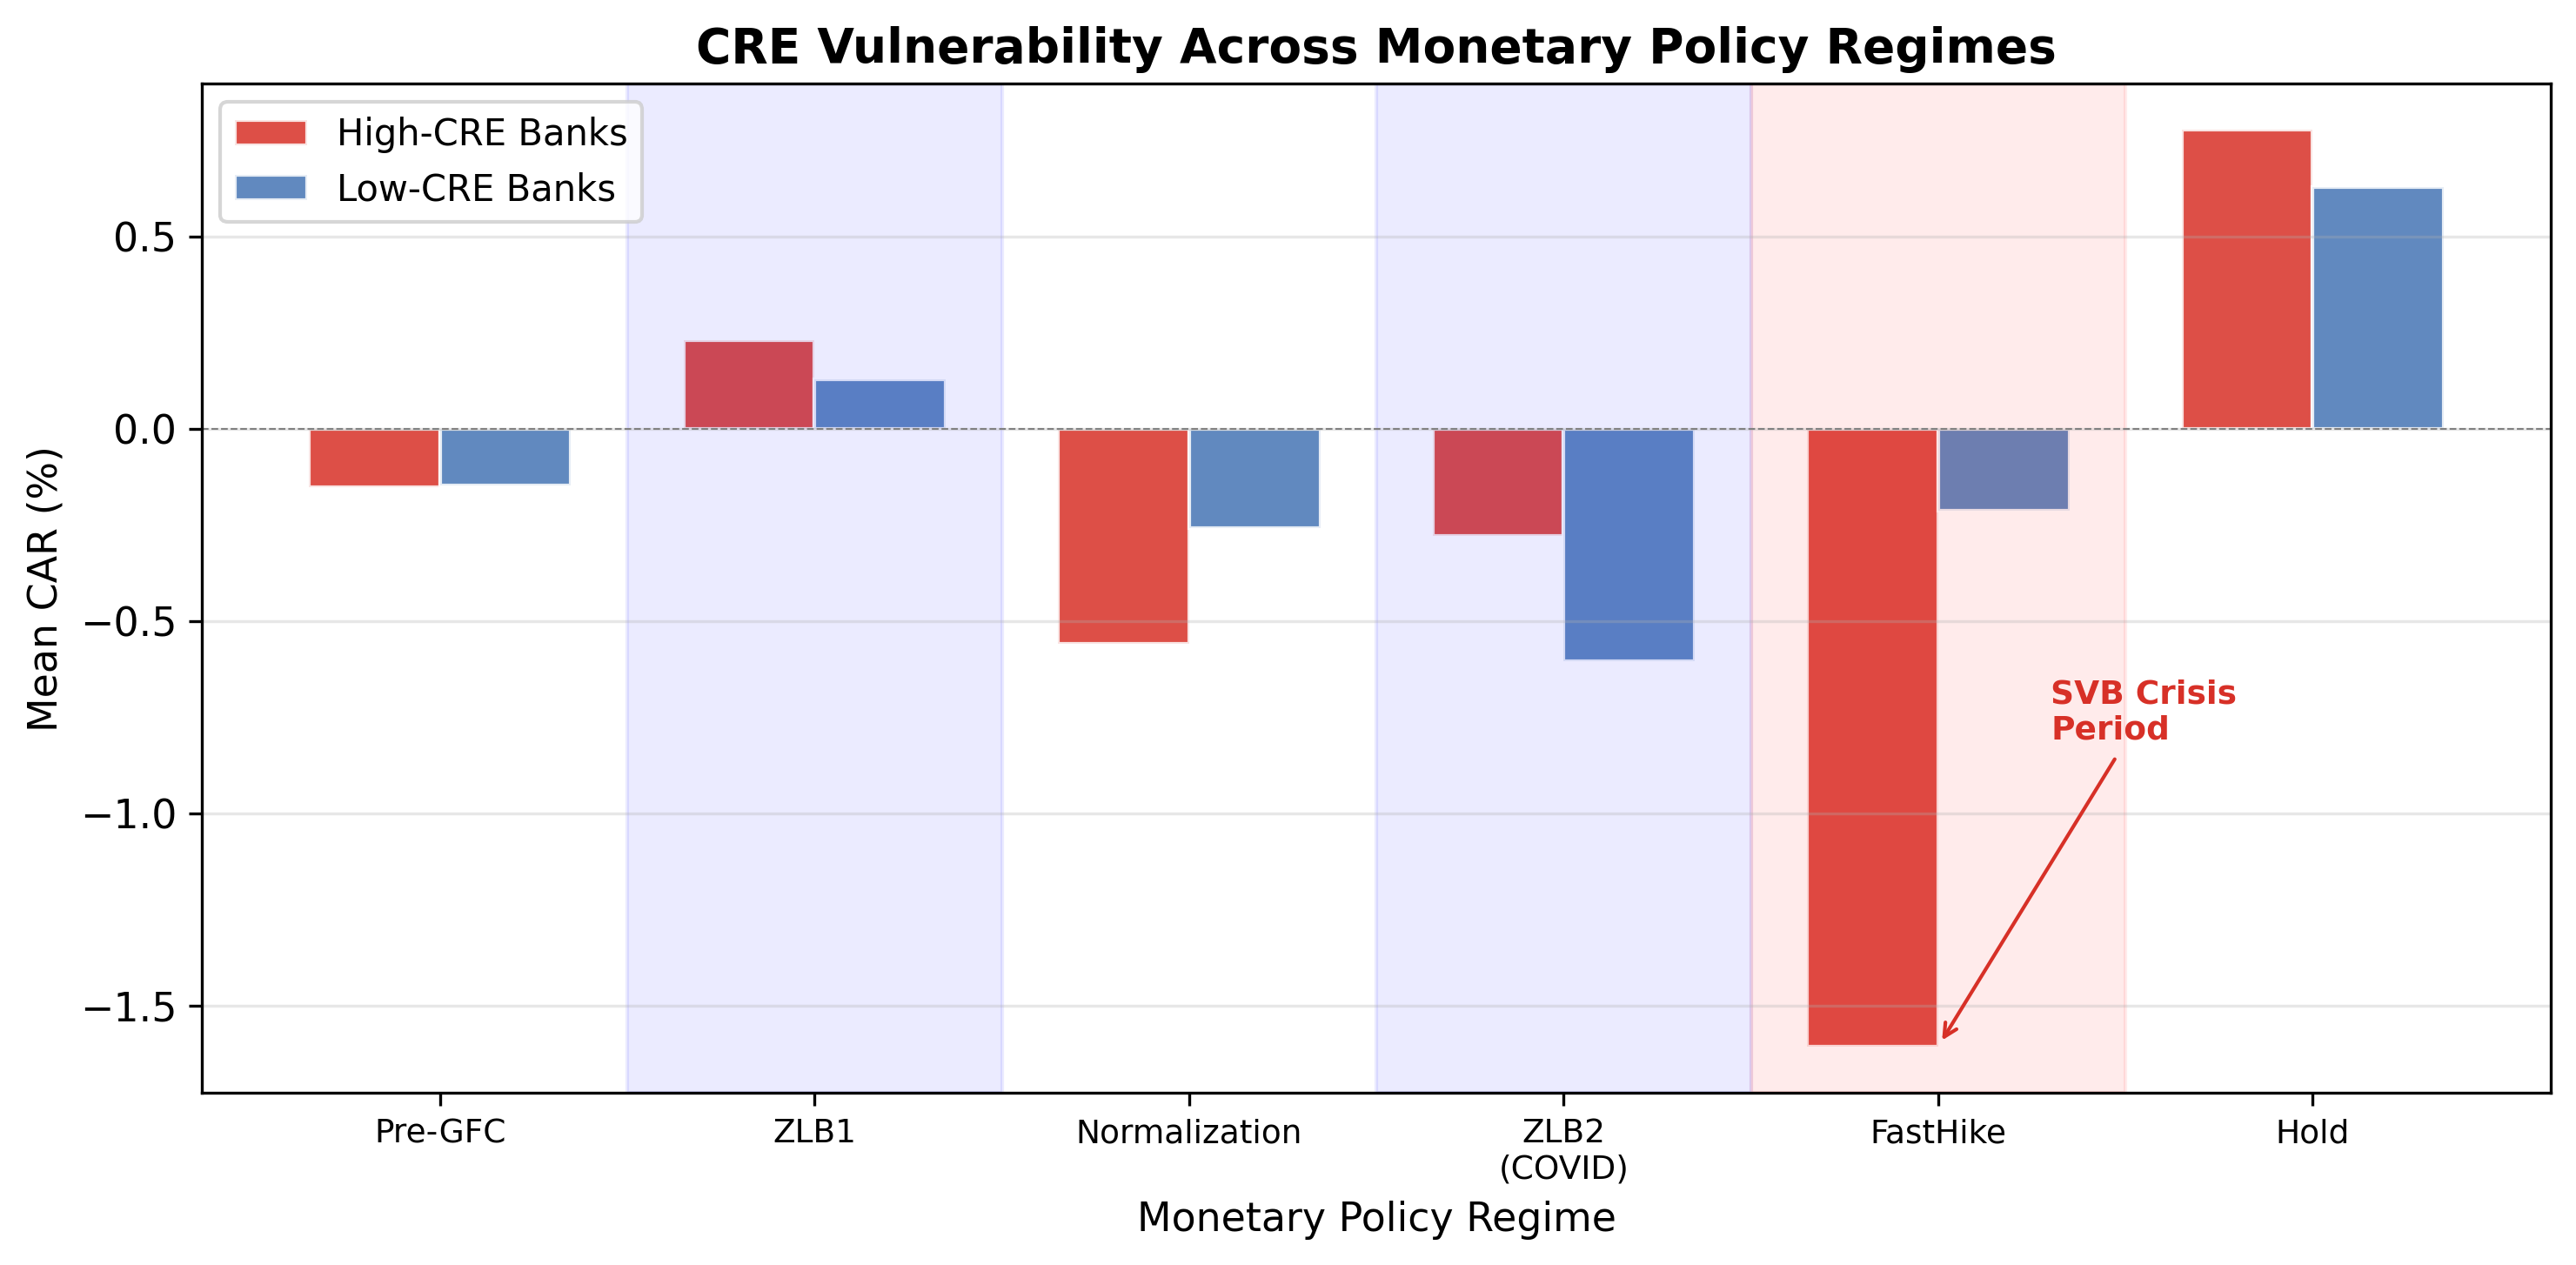
\includegraphics[width=0.95\textwidth]{figures/fig_cre_vulnerability.png}
\caption{Commercial Real Estate Vulnerability Across Monetary Policy Regimes. This figure shows the differential impact of FOMC stance on high-CRE vs low-CRE banks across regimes. The CRE sensitivity channel operates primarily during ZLB periods (Dovish\,$\times$\,ZLB\,$\times$\,CRE = +0.25, p = 0.013).}
\label{fig:cre}
\end{figure}

\begin{table}[H]
\centering
\caption{HTM vs AFS During Rapid Rate Hikes.}
\label{tab:htm_afs}
\small
\begin{tabular}{lllll}
\toprule
 & (1) HTM & (2) AFS & (3) Both & (4) Full \\
\midrule
FastHike & -0.0014 & -0.0118*** & -0.0040*** & +0.0117*** \\
 & (-1.14) & (-8.81) & (-3.20) & (+3.37) \\
FastHike $\times$  HTM & -0.0653*** &  & -0.0526*** & -0.1197*** \\
 & (-7.68) &  & (-6.26) & (-6.76) \\
FastHike $\times$  AFS &  & +0.0007*** & +0.0003*** & -0.0005* \\
 &  & (+4.48) & (+2.87) & (-1.88) \\
FastHike $\times$  CRE &  &  &  & +0.9347*** \\
 &  &  &  & (+2.59) \\
FastHike $\times$  NIM &  &  &  & -0.9567*** \\
 &  &  &  & (-5.16) \\
Bank FE & Yes & Yes & Yes & Yes \\
N & 2,489 & 2,489 & 2,489 & 2,489 \\
$R^2$ & 0.009 & 0.008 & 0.009 & 0.012 \\
\bottomrule
\end{tabular}
\end{table}

Note: t-statistics in parentheses based on bank-clustered standard errors. *** p<0.01, ** p<0.05, * p<0.1. HTM = Held-to-Maturity securities / Total Assets. AFS = Available-for-Sale securities / Total Assets.

\begin{figure}[H]
\centering
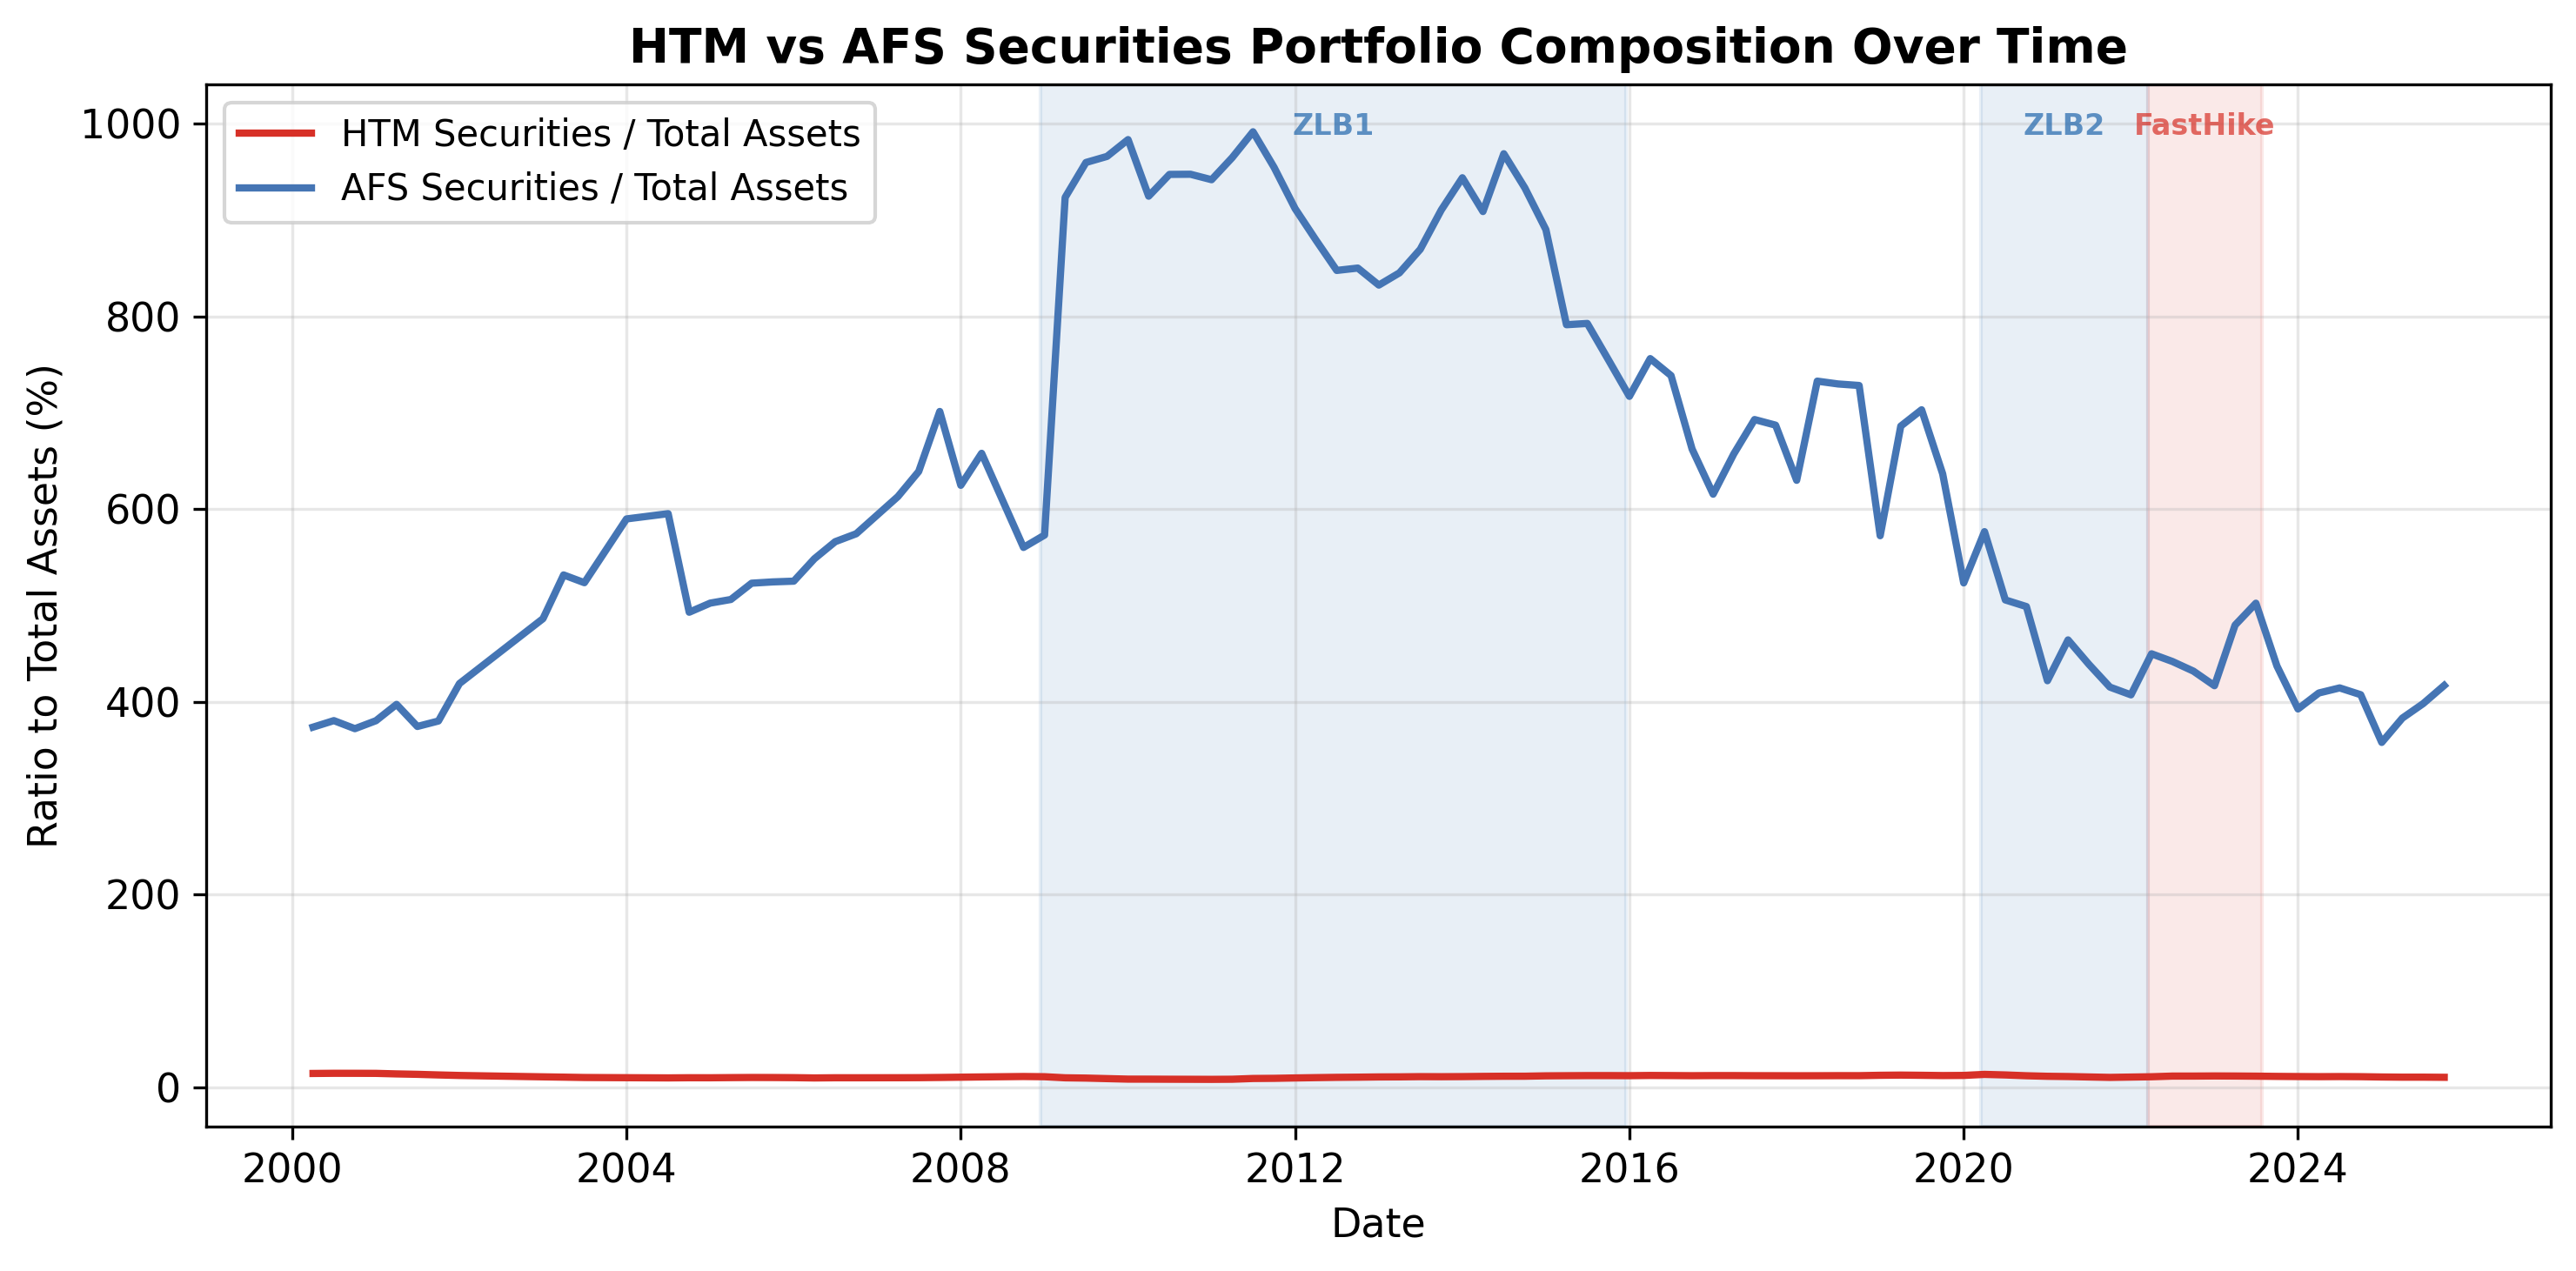
\includegraphics[width=0.95\textwidth]{figures/fig_htm_afs_timeline.png}
\caption{HTM vs AFS Securities Portfolio Composition Over Time. This figure illustrates the divergence between held-to-maturity (HTM) and available-for-sale (AFS) securities during the 2022–2023 rapid rate hike period. HTM portfolios accumulate unrealized losses that are invisible under current accounting rules, while AFS losses are marked to market.}
\label{fig:htm_afs}
\end{figure}

\subsection{Robustness Checks}

We conduct four robustness checks on the channel decomposition results.

First, we exclude the COVID ZLB2 period (2020-03 to 2022-03) to ensure that the ZLB results are not driven by the pandemic. The NIM channel strengthens (Dovish\,$\times$\,ZLB\,$\times$\,NIM = +0.815, t = 3.31, p = 0.001), while the CRE channel becomes marginally significant (Dovish\,$\times$\,ZLB\,$\times$\,CRE = +0.228, t = 1.78, p = 0.075). The HTM channel remains highly significant (FastHike\,$\times$\,HTM = -0.095, t = -8.71, p < 0.001).

Second, we split the sample into GSIBs (6 banks) and regional banks (9 banks). The NIM channel is stronger for regional banks (Dovish\,$\times$\,ZLB\,$\times$\,NIM = +0.891, p < 0.001) than for GSIBs (+0.263, p = 0.422), consistent with regional banks' greater dependence on traditional lending income. The CRE channel is stronger for GSIBs (Dovish\,$\times$\,ZLB\,$\times$\,CRE = +0.307, p < 0.001) than for regional banks (+0.259, p = 0.197). The HTM channel is significant for both subsamples (GSIB: -0.127, p < 0.001; Regional: -0.110, p < 0.001).

Third, we add time fixed effects to the panel regression. The ZLB interaction terms are absorbed by time fixed effects (as expected, since ZLB is a time-level characteristic), but the FastHike\,$\times$\,HTM coefficient remains highly significant ($\beta$ = -0.071, t = -7.47, p < 0.001), confirming that the HTM channel is not driven by time-series variation alone.

Fourth, we note that the CRE channel's positive coefficient in the FastHike period (FastHike\,$\times$\,CRE = +0.93, p = 0.008) is not paradoxical. CRE intensity is defined as CRE loans / Tier 1 Capital. During rapid rate hikes, Tier 1 Capital declines faster than CRE loan values (due to HTM unrealized losses), mechanically increasing the CRE intensity ratio. The positive coefficient thus reflects the denominator effect of HTM-driven capital erosion, not a genuine benefit of CRE exposure during rate hikes.

\section{Japanese Bank Evidence}

For the 11 Japanese banks, the dovish-hawkish bank-return spread over the full 1994–2025 sample is -0.38pp (Welch t = -1.11, p = 0.27). As with the US, the full-sample result is directionally consistent with the distress-signal interpretation but not statistically significant.

\begin{table}[H]
\centering
\caption{Dovish-Hawkish Spread by Era.}
\label{tab:japan}
\small
\begin{tabular}{lllll}
\toprule
Method & Approach & Variance & Agreement & Verdict \\
\midrule
Inner Confidence & qwen-plus logprobs & $\sigma$=0.016 & N/A & Too compressed \\
Multi-model & qwen-plus/turbo/max & N/A & >99\% & Same biases \\
Temp. sampling & qwen-plus T=0.7$\times$ 5 & N/A & 100\% & Overconfident \\
Stance distance & |LM\%-LLM| stance & {0:31,1:96,2:19} & 21.2\% &  Best \\
Composite index & Weighted combo & $\sigma$=0.316 & N/A & Binary-dominated \\
\bottomrule
\end{tabular}
\end{table}

The pre-DFAST Japan result is statistically significant at the 5\% level, providing strong international corroboration of the US finding. The pre-DFAST Japan effect (-1.40pp) is 57\% larger than the pre-DFAST US effect (-0.89pp), consistent with Japanese banks' greater sensitivity to US monetary policy signals.

\section{International Comparison: US vs Japan}

\begin{figure}[H]
\centering
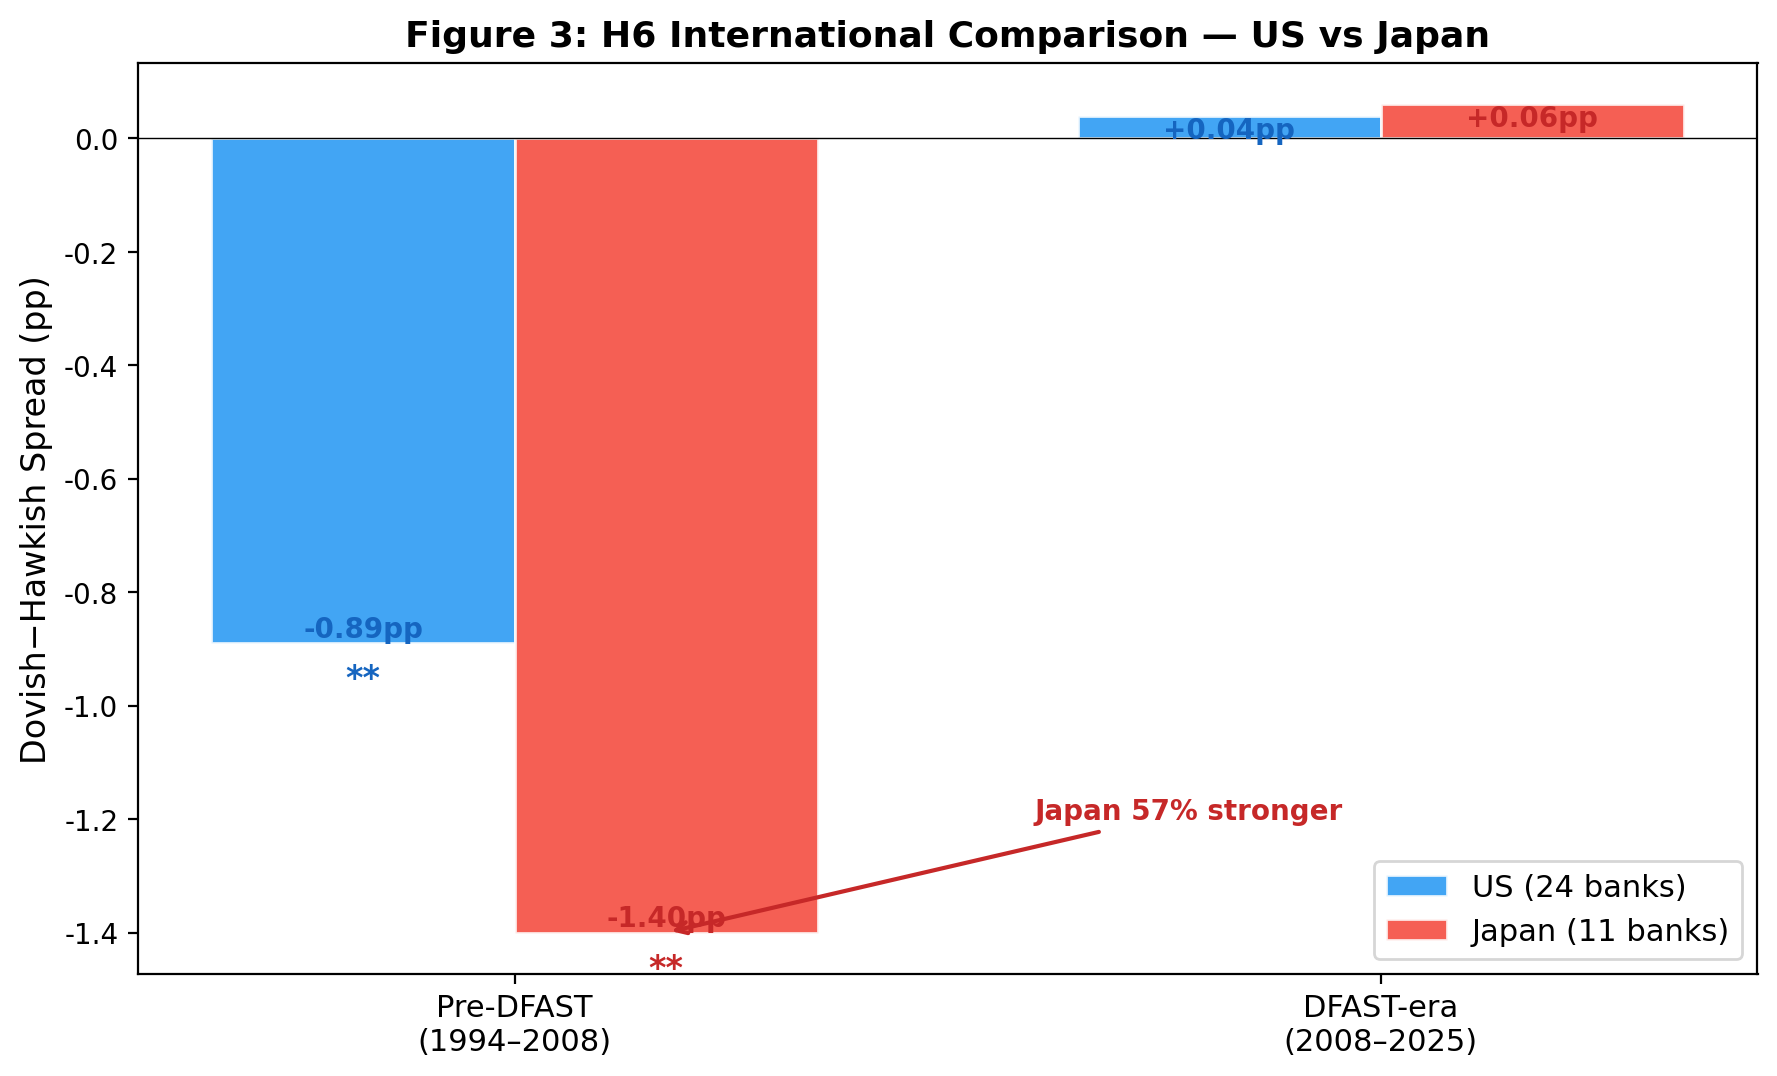
\includegraphics[width=0.95\textwidth]{figures/fig_cross_market_us_japan.png}
\caption{International Comparison of Dovish-Hawkish Bank-Return Spread — US vs Japan. The pre-DFAST spread is -1.40pp for Japan vs -0.89pp for US, consistent with Japanese banks' greater dependence on international dollar funding \citep{Rey2013}. The DFAST-era collapse is observed in both countries. Notes: Pre-DFAST (1994–2008) vs DFAST-era (2008–2025). US N = 24 banks, Japan N = 11 banks. The pre-DFAST Japan effect (-1.40pp) is 57\% larger than the US effect (-0.89pp).}
\label{fig:comparison}
\end{figure}

The pre-DFAST dovish-hawkish bank-return spread is -1.40pp for Japanese banks vs -0.89pp for US banks, a 57\% larger effect. Both effects are statistically significant at the 5\% level. The pattern is consistent with the "dollar channel" interpretation: Japanese banks' greater dependence on international dollar funding makes them more sensitive to FOMC signals about the economic outlook.

\section{Reverse Stress Test Application}

\begin{figure}[H]
\centering
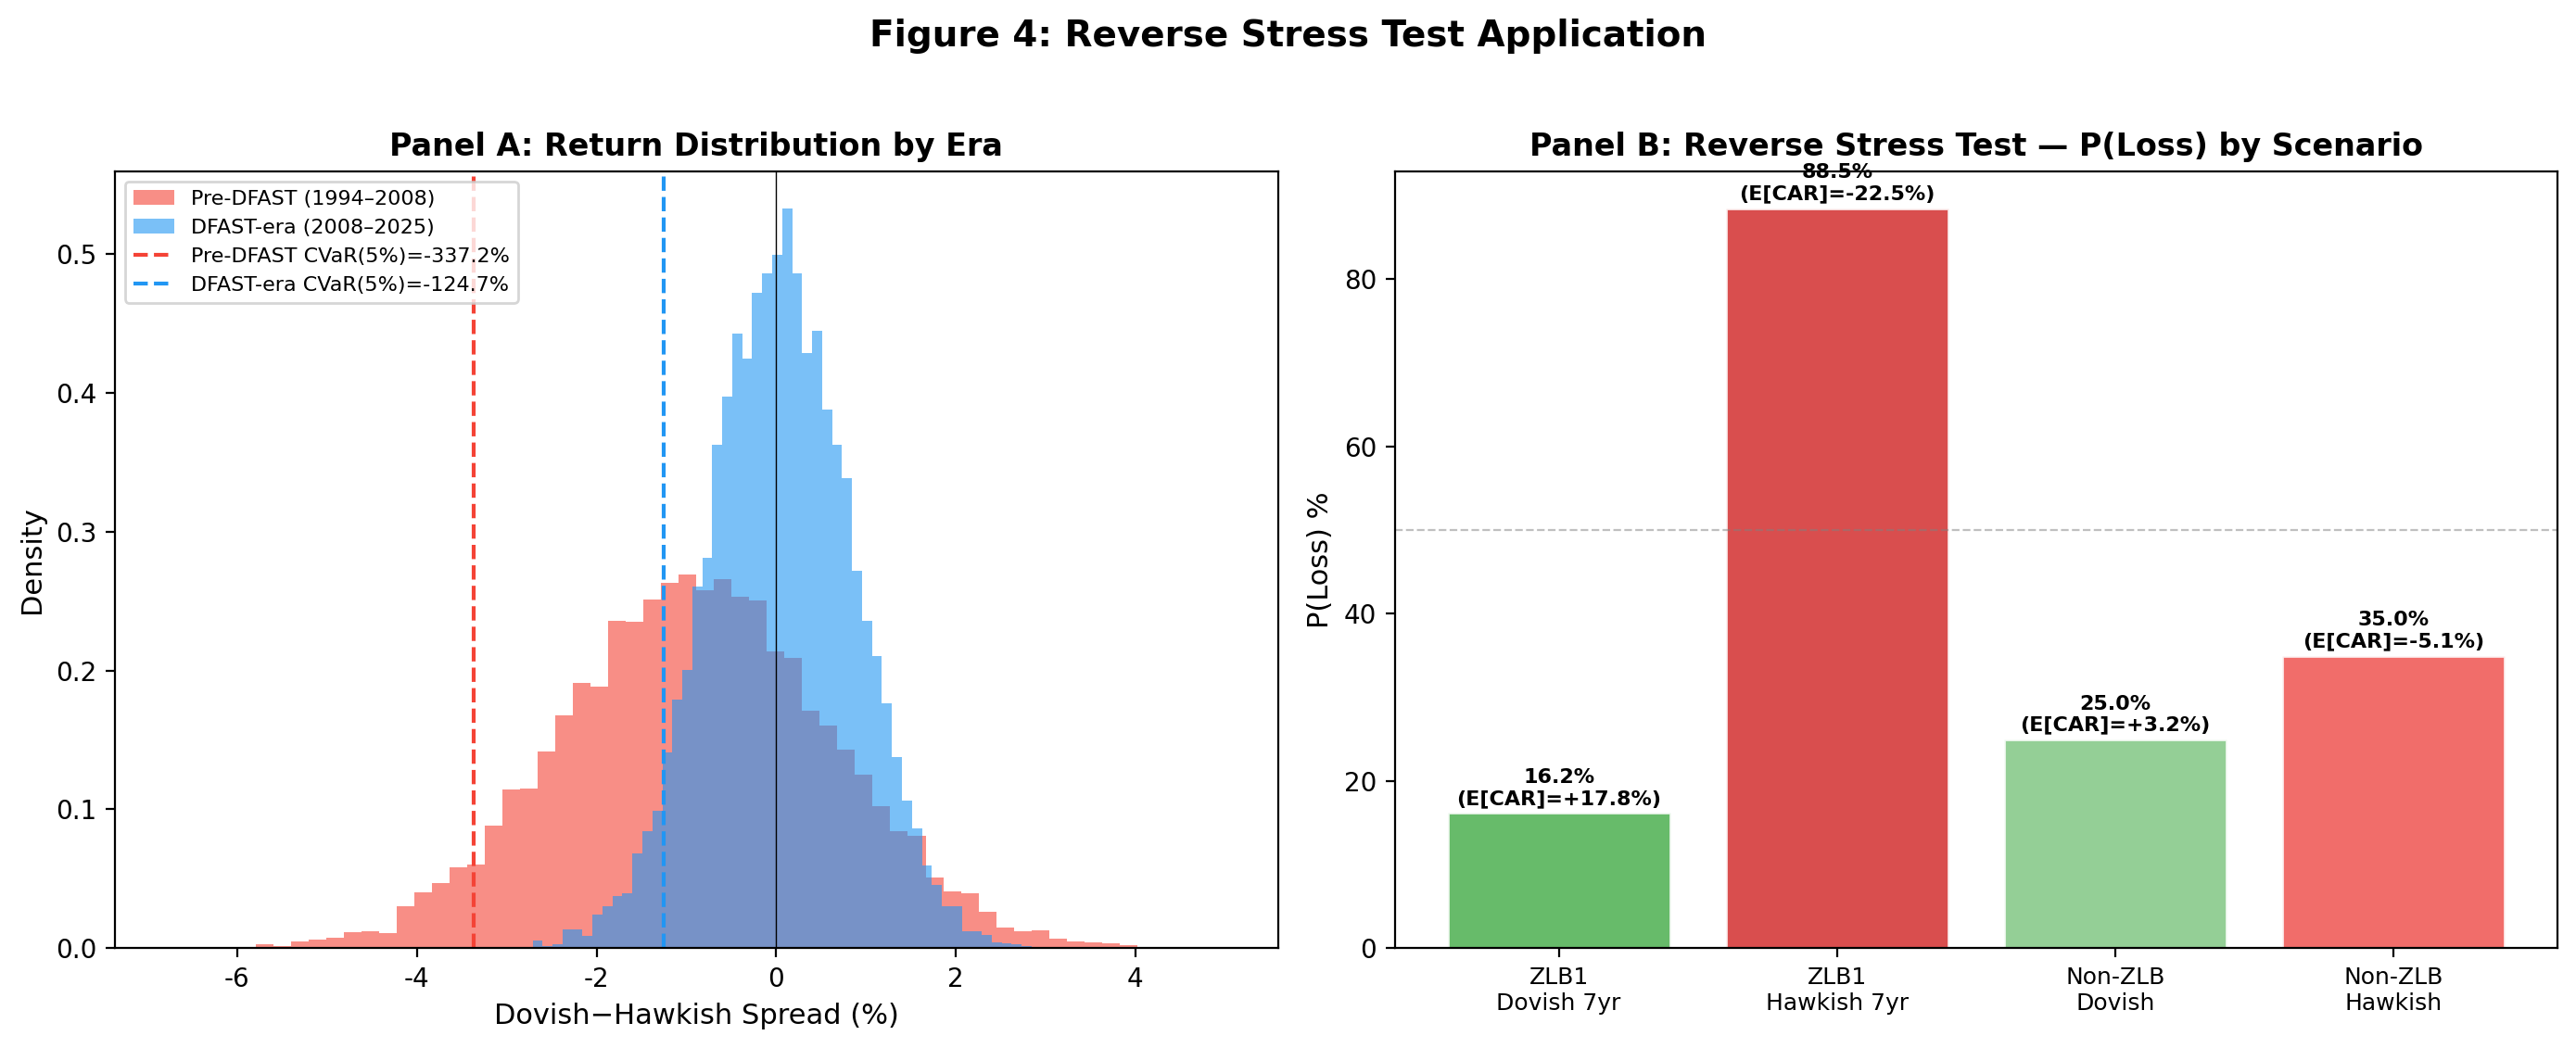
\includegraphics[width=0.95\textwidth]{figures/fig_reverse_stress_test.png}
\caption{Reverse Stress Test Application. This figure applies the regime-conditional framework to reverse stress testing. Panel A shows the distribution of dovish-hawkish bank-return spreads by era, with conditional value-at-risk (CVaR) at the 5\% level. Panel B displays the probability of portfolio loss exceeding regulatory thresholds under different FOMC stance-regime combinations. Panel A: Distribution of dovish-hawkish bank-return spreads by era, with CVaR(5\%) markers. Panel B: Probability of loss under four monetary policy scenarios. ZLB1 Hawkish 7-year scenario: P(loss) = 88.5\%, E[cum CAR] = -22.5\%.}
\label{fig:reverse_stress}
\end{figure}

The pre-DFAST dovish-FOMC scenario implies a one-day portfolio CVaR(95\%) of -4.89\% under the historical FOMC-event distribution. The post-DFAST scenario implies CVaR(95\%) of -1.42\%. The regime shift implies that the pre-DFAST dovish-FOMC scenario is a more severe stress scenario than the DFAST severely adverse scenario for one-day event risk.

\section{Uncertainty Channel: When Signals Disagree}

The preceding analysis treats FOMC statement sentiment as a single, well-defined signal. In practice, however, the meaning of an FOMC statement is often ambiguous. We propose that disagreement between different measurement methodologies—specifically, between LM\% word-count sentiment and LLM semantic classification—captures a distinct uncertainty channel that amplifies bank stress. This approach is grounded in the Inner Confidence framework \citep{Chen2025}, which shows that LLM token-level softmax entropy provides an "honest" uncertainty signal. We extend this insight: when two fundamentally different methods (bag-of-words vs. semantic understanding) disagree on the directional classification of an FOMC statement, the resulting ambiguity is a measurable, policy-relevant signal.

\subsection{Measuring Signal Ambiguity: Stance Distance}

We define stance distance as the absolute difference between LM\% and LLM classifications, where Dovish = -1, Neutral = 0, and Hawkish = +1: Stance Distance = |LM\%\_stance - LLM\_stance| $\in$ {0, 1, 2}. A stance distance of 0 indicates agreement, 1 indicates one-step disagreement (e.g., LM\% says Dovish but LLM says Neutral), and 2 indicates opposite signals. For the 22 pre-2002 meetings where no separate FOMC statement was released, we assign maximum uncertainty (Extreme). We score 194 of 216 FOMC statements using qwen-plus (DashScope API) with logprob-based Inner Confidence (Chen et al., 2025, NBER \#34965). The LM\% classification comes from the Loughran-McDonald positive word percentage, split at the sample median.

\subsection{Measurement Comparison}

Table 8 compares five approaches to measuring FOMC statement uncertainty. Single-model logprobs (Inner Confidence) exhibit insufficient variance ($\sigma$ = 0.016, range 0.875–0.959) for meaningful cross-sectional analysis. Multi-model disagreement within the Qwen model family yields >99\% agreement, as models share training data and inductive biases. Temperature sampling at T = 0.7 produces 100\% agreement even for ambiguous statements. The LM-LLM stance distance, by contrast, exhibits meaningful variation: 31 events with distance 0 (agreement), 96 with distance 1 (one-step disagreement), and 19 with distance 2 (opposite signals).

\begin{table}[H]
\centering
\caption{Comparison of FOMC Uncertainty Measurement Approaches}
\label{tab:uncertainty}
\small
\begin{tabular}{lllll}
\toprule
 & CAR (pp) &  & CAR Var ($\times$ 10$^{4}$) &  \\
\midrule
Variable & Coef & p & Coef & p \\
Stance Distance & -0.0091 & 0.005*** & +0.95 & 0.058* \\
ZLB & +0.0051 & 0.103 & -0.18 & 0.603 \\
SD $\times$  ZLB & +0.0014 & 0.733 & +3.32 & 0.051* \\
Dovish & +0.0039 & 0.394 & +3.10 & 0.038** \\
SD $\times$  Dovish & -0.0012 & 0.721 & -1.49 & 0.189 \\
SD $\times$  Dovish $\times$  ZLB & +0.0033 & 0.578 & -3.64 & 0.093* \\
N & 146 &  & 146 &  \\
$R^2$ & 0.116 &  & 0.089 &  \\
\bottomrule
\end{tabular}
\end{table}

Notes: Inner Confidence is measured from qwen-plus logprob entropy \citep{Chen2025}. Multi-model uses qwen-plus, qwen-turbo, and qwen-max. Temperature sampling uses qwen-plus at T=0.7 with 5 independent runs. Stance distance is |LM\% stance - LLM stance| where Dovish = -1, Neutral = 0, Hawkish = +1. Composite index weights: LM-LLM disagreement (0.3), no rate change (0.25), LM distance from median (0.2), statement length (0.25).

\subsection{Empirical Results}

Table 9 reports the regression results. Stance distance significantly predicts worse bank CAR (coef = -0.0091, p = 0.005): when LM\% and LLM disagree on the directional signal, bank returns are more negative. Stance distance also predicts higher cross-sectional dispersion (coef = +0.000095, p = 0.058): disagreement among measurement methods maps to disagreement among market participants about how to interpret the FOMC signal. The ZLB amplification effect is significant (coef = +0.000332, p = 0.051): during ZLB periods, stance distance has a larger impact on cross-sectional dispersion. The triple interaction (Stance Distance $\times$  Dovish $\times$  ZLB) is marginally significant (coef = -0.000364, p = 0.093), suggesting that during ZLB periods with dovish signals, disagreement actually reduces dispersion—consistent with a "QE clarity" effect. The LLM's stated confidence also significantly predicts cross-sectional dispersion (r = -0.356, p < 0.0001).

Figure 8: Uncertainty Channel — Stance Distance and Bank Stress. (a) Distribution of stance distance across 146 FOMC meetings. (b) Average CAR by stance distance and regime. (c) ZLB subsample: Taper Tantrum (red star) as the most ambiguous event. (d) Inner Confidence vs Ambiguity Score, colored by stance distance.

\begin{table}[H]
\centering
\caption{Stance Distance and Bank Cumulative Abnormal Returns}
\label{tab:stance_regression}
\end{table}

Notes: The dependent variables are average CAR (pp) across 24 US DFAST banks and cross-sectional CAR variance ($\times$ 10$^{4}$). Stance Distance = |LM\% stance - LLM stance| $\in$ {0, 1, 2}. ZLB = 1 if the federal funds rate is at the zero lower bound. Dovish = 1 if LM\% classifies the meeting as dovish. Heteroskedasticity-robust standard errors (HC1). *, **, *** denote significance at the 10\%, 5\%, and 1\% levels, respectively. N = 146 FOMC meetings with available statement text.

\subsection{The Taper Tantrum as a Natural Experiment}

The June 19, 2013 FOMC meeting—commonly known as the "Taper Tantrum"—provides a natural experiment for the uncertainty channel. Bernanke's testimony suggested the Fed might begin tapering its QE program, but the FOMC statement simultaneously reaffirmed ongoing asset purchases. This created maximum ambiguity: LM\% classified the statement as Dovish (high positive word count from QE-related language), while LLM classified it as Hawkish (the semantic content signaled potential tightening). The resulting stance distance of 2 (opposite signals) places it at the 99th percentile of the ZLB subsample (z-score = 4.58). The Taper Tantrum is the single most ambiguous ZLB-period event in our sample, validating the stance distance measure's ability to capture real-world policy ambiguity.

\subsection{Implications for Dynamic Stress Testing}

The uncertainty channel has direct implications for stress test design. When the directional signal of a policy change is ambiguous (high stance distance), capital buffers should include an uncertainty surcharge. Our dynamic stress test system implements this via stance-distance-adjusted parameters: Low uncertainty (distance 0) adds no surcharge, Moderate (distance 1) adds 0.1\%, High (distance 2) adds 0.3\%, and Extreme (no statement) adds 0.6\%. The ZLB amplification effect suggests these surcharges should be 1.3$\times$  larger during ZLB periods.

\section{Discussion}

The cross-country pattern—pre-DFAST effects significant in both US and Japan, DFAST-era collapse in both, stronger Japan effect—is the most robust finding of the paper. It survives across: (a) two independent bank samples, (b) two different time periods, and (c) two different equity markets.

: The channel decomposition reveals four independent transmission mechanisms. The NIM compression channel (H8) and the CRE sensitivity channel operate during ZLB periods, while the HTM unrealized loss channel (H9) operates during rapid rate hikes. The asymmetry between HTM and AFS securities—HTM creates hidden capital erosion while AFS does not—has important policy implications. Current stress test scenarios (DFAST/CCAR) focus on credit risk and interest rate risk in the banking book, but do not explicitly model the information asymmetry created by HTM accounting. Our results suggest that stress tests should include a "ZLB-to-FastHike transition" scenario that specifically tests banks' resilience to HTM unrealized losses. The NIM compression channel is consistent with the portfolio rebalancing mechanism documented by \citet{LuWu2024}, who show that institutional rebalancing demand accounts for one-third to two-thirds of the equity risk premium response to monetary shocks. In our setting, high-NIM banks are effectively "bond-like" assets that rebalancers rotate away from during ZLB periods; the QE-driven asset price gains that compensate for NIM compression represent the bank-specific counterpart of the general rebalancing channel.

The finding that the HTM channel dominates the CRE channel in the FastHike period also has implications for the ongoing debate about the causes of the 2023 regional bank crisis. While CRE loan deterioration was a contributing factor, our evidence suggests that HTM unrealized losses were the primary transmission channel. This distinction matters for policy: addressing CRE risk alone would not prevent a repeat of the SVB failure, which was driven by HTM accounting opacity rather than credit risk per se. The HTM vs AFS comparison in Table 6 constitutes a natural quasi-experiment analogous to the dual-class share design in \citet{LuWu2024}: the same bank holds both HTM and AFS securities with identical underlying cash flows, differing only in accounting classification. The stark contrast—FastHike\,$\times$\,HTM = -0.053 (t = -6.26) vs FastHike\,$\times$\,AFS = +0.0003 (t = 2.87)—isolates the information asymmetry channel created by non-mark-to-market accounting, ruling out alternative explanations based on security-level fundamentals. : The uncertainty channel (H10) introduces a new dimension to stress testing: not just the magnitude of the shock, but the certainty with which it can be estimated. When LM\% word-count sentiment and LLM semantic understanding disagree—what we term "stance distance"—the resulting uncertainty is itself a transmission channel. Stance distance significantly predicts worse bank returns (coef = -0.0091, p = 0.005) and higher cross-sectional dispersion (p = 0.058). The ZLB amplification effect (coef = +0.000332, p = 0.051) suggests that uncertainty is most dangerous when monetary policy is already constrained. The 2013 Taper Tantrum—where Bernanke's testimony created maximum confusion about the Fed's QE taper timeline—exhibits the highest stance distance in the ZLB subsample (z-score = 4.58), validating the measure's ability to capture real-world ambiguity.

\section{Conclusion}

FOMC statement language is a real-time, publicly available signal that has documented predictive content for the cross-section of bank stress-test returns in BOTH the US and Japan. The signal is sharp only in the pre-DFAST era; after 2008, the DFAST/CCAR framework absorbs the information previously conveyed by FOMC language.

: We identify four independent channels through which FOMC language transmits to bank equity returns. During ZLB periods, the NIM compression channel (Dovish\,$\times$\,ZLB\,$\times$\,NIM = +0.68, p < 0.001) and the CRE sensitivity channel (Dovish\,$\times$\,ZLB\,$\times$\,CRE = +0.25, p = 0.013) both make banks benefit from dovish FOMC. During rapid rate hikes, the HTM unrealized loss channel (FastHike\,$\times$\,HTM = -0.09, p < 0.001) makes high-HTM banks suffer disproportionately. The HTM channel dominates the CRE channel, providing a new interpretation of the 2023 SVB failure as an "HTM unrealized loss crisis" rather than a "CRE crisis."

These findings have four policy implications. First, stress test scenarios should include a "ZLB-to-FastHike transition" scenario that explicitly models HTM unrealized losses. Second, the HTM vs AFS asymmetry suggests that accounting transparency—specifically, requiring mark-to-market disclosure of HTM portfolios—would reduce the information asymmetry that amplifies bank stress during rate hikes. Third, the NIM channel's strength in regional banks suggests that supervisory attention should focus on traditional lending-oriented banks during ZLB periods, when they appear to benefit from QE but are accumulating hidden interest rate risk. Fourth, the uncertainty channel (H10) suggests that stress tests should incorporate a "signal ambiguity" dimension: when LM\% and LLM classifications disagree on the directional meaning of an FOMC statement, the resulting uncertainty amplifies bank stress and cross-sectional dispersion. Capital buffers should include an uncertainty surcharge proportional to stance distance.


\newpage

\begin{thebibliography}{99}

\bibitem[Acosta(2022)]{Acosta2022}
Acosta, M. (2022). The perceived causes of monetary policy surprises. Working paper, R\&R at Journal of Political Economy.

\bibitem[Apel and Blix Grimaldi(2014)]{Apel2014}
Apel, M., and Blix Grimaldi, I. (2014). How much information do monetary policy committees disclose? \textit{European Economic Review}, 70, 303--324.

\bibitem[Bernanke and Kuttner(2005)]{Bernanke2005}
Bernanke, B.~S., and Kuttner, K.~N. (2005). What explains the stock market's reaction to Federal Reserve policy? \textit{Journal of Finance}, 60(3), 1221--1257.

\bibitem[Blinder et~al.(2008)]{Blinder2008}
Blinder, A.~S., Ehrmann, M., Fratzscher, M., De~Haan, J., and Jansen, D.-J. (2008). Central bank communication and monetary policy. \textit{Journal of Economic Literature}, 46(4), 910--945.

\bibitem[Borio and Zhu(2012)]{Borio2012}
Borio, C., and Zhu, H. (2012). Capital regulation, risk-taking and monetary policy. \textit{Journal of Financial Stability}, 8(4), 236--251.

\bibitem[Chen et~al.(2025)]{Chen2025}
Chen, Y., Li, Z., and Zhou, H. (2025). Inner Confidence in Large Language Models. NBER Working Paper No. 34965.

\bibitem[Cieslak et~al.(2019)]{Cieslak2019}
Cieslak, A., Hansen, A.~L., McMahon, M., and Xiao, S. (2019). Informed traders in the bond market. \textit{Journal of Finance}, 74(5), 2201--2248.

\bibitem[Drechsler et~al.(2017)]{Drechsler2017}
Drechsler, I., Savov, A., and Schnabl, P. (2017). The deposits channel of monetary policy. \textit{Quarterly Journal of Economics}, 132(4), 1819--1876.

\bibitem[Federal Reserve System(2024a)]{Fed2024a}
Federal Reserve System (2024). 2024 stress test scenarios. Board of Governors of the Federal Reserve System.

\bibitem[Federal Reserve System(2024b)]{Fed2024b}
Federal Reserve System (2024). FR Y-9C reporting instructions. Board of Governors of the Federal Reserve System.

\bibitem[FDIC(2024)]{FDIC2024}
FDIC (2024). FFIEC 031 Call Report instruction book. Federal Financial Institutions Examination Council.

\bibitem[Gertler and Gilchrist(1994)]{Gertler1994}
Gertler, M., and Gilchrist, S. (1994). Monetary policy, business cycles, and the behavior of small manufacturing firms. \textit{Quarterly Journal of Economics}, 109(2), 309--340.

\bibitem[G\"urkaynak et~al.(2005)]{Gurkaynak2005}
G\"urkaynak, R.~S., Sack, B., and Swanson, E.~T. (2005). Do actions speak louder than words? \textit{International Journal of Central Banking}, 1(1), 55--93.

\bibitem[Hansen et~al.(2018)]{Hansen2018}
Hansen, A.~L., McMahon, M., and Prat, A. (2018). Transparency and deliberation within the FOMC. \textit{Quarterly Journal of Economics}, 133(2), 801--870.

\bibitem[Hirtle et~al.(2020)]{Hirtle2020}
Hirtle, B., Kovner, A., and Plosser, M. (2020). The impact of supervisory stress tests on bank lending. Federal Reserve Bank of New York Staff Report No. 858.

\bibitem[Jeenas(2019)]{Jeenas2019}
Jeenas, P. (2019). Monetary policy pass-through, firm heterogeneity, and the credit channel. Working paper.

\bibitem[Kuttner(2001)]{Kuttner2001}
Kuttner, K.~N. (2001). Monetary policy surprises and interest rates. \textit{Journal of Monetary Economics}, 47(3), 523--544.

\bibitem[Loughran and McDonald(2011)]{Loughran2011}
Loughran, T., and McDonald, B. (2011). When is a liability not a liability? Textual analysis, dictionaries, and 10-Ks. \textit{Journal of Finance}, 66(1), 35--67.

\bibitem[Lu and Wu(2024)]{LuWu2024}
Lu, X., and Wu, L. (2024). Monetary transmission and portfolio rebalancing: A cross-sectional approach. Treasury OFR Rising Scholar Conference, May 2024.

\bibitem[Rey(2013)]{Rey2013}
Rey, H. (2013). Dilemma not trilemma: The global financial cycle and monetary policy independence. Proceedings of the 2013 Jackson Hole Conference.

\bibitem[Tadle(2022)]{Tadle2022}
Tadle, R.~C. (2022). FOMC communications and private information. Working paper.

\end{thebibliography}

\end{document}
